% ===================================================================
%  LG-CISH - FULL PAPER (major). Build: pdflatex lgcish_academic.tex (x2).
%  Inline: Introduction, Related Work, Proposed Method, Discussion, Conclusion.
%  Modular \input: algorithms.tex (Alg 1-5) and lgcish_results.tex (results).
%  Figures from ./figures/. Conventions: passive voice,
%  "Figure~\ref" and "Equation~\eqref".
% ===================================================================
\documentclass[11pt]{article}
\usepackage[margin=1in]{geometry}
\usepackage{amsmath,amssymb,amsthm,mathtools}
\usepackage{graphicx}
\usepackage{booktabs}
\usepackage{float}
\usepackage{xcolor}
\usepackage{caption}
\usepackage{etoolbox}
\usepackage{ragged2e}
\usepackage{titlesec}
\usepackage{tikz}
\usetikzlibrary{positioning,arrows.meta,calc,fit,shapes.geometric,backgrounds}
\usepackage[hidelinks]{hyperref}
\usepackage[section]{placeins}

\graphicspath{{./figures/}}
\def\LGCISHMAIN{}   % tells lgcish_results.tex it is being \input, not standalone

% --- document alignment and typography ---
\setcounter{secnumdepth}{3}
\titleformat{\section}
  {\normalfont\Large\bfseries\raggedright}{\thesection}{1em}{}
\titleformat{\subsection}
  {\normalfont\large\bfseries\raggedright}{\thesubsection}{1em}{}
\titleformat{\subsubsection}
  {\normalfont\normalsize\bfseries\raggedright}{\thesubsubsection}{1em}{}
\titleformat{\paragraph}[runin]
  {\normalfont\normalsize\bfseries}{\theparagraph}{1em}{}
\captionsetup{font=normalsize,justification=centering,singlelinecheck=false}
\AtBeginEnvironment{table}{\centering}
\AtBeginEnvironment{figure}{\centering}
\AtBeginEnvironment{thebibliography}{\fontsize{12}{14.4}\selectfont}
\AtBeginDocument{\justifying}

% Left-aligned abstract heading with justified abstract text.
\renewenvironment{abstract}{%
  \par\noindent\textbf{\abstractname}\par\medskip\justifying
}{\par\medskip}

% --- theorem-like environments ---
\theoremstyle{definition}
\newtheorem{definition}{Definition}[section]
\newtheorem{assumption}{Assumption}[section]
\newtheorem{proposition}{Proposition}[section]

% --- self-contained algorithm float + pseudocode ---
\floatstyle{ruled}
\newfloat{algorithm}{tbp}{loa}
\floatname{algorithm}{Algorithm}
\newcounter{algln}
\newenvironment{pseudo}{%
  \begin{list}{\footnotesize\arabic{algln}:}{%
    \usecounter{algln}%
    \setlength{\leftmargin}{2.4em}\setlength{\labelwidth}{1.7em}%
    \setlength{\labelsep}{0.4em}\setlength{\itemsep}{1.5pt}%
    \setlength{\parsep}{0pt}\setlength{\topsep}{3pt}\small}%
}{\end{list}}
\newcommand{\kw}[1]{\textbf{#1}}
\newcommand{\Ind}{\hspace*{1.3em}}
\newcommand{\Indd}{\hspace*{2.6em}}
\newcommand{\Cmt}[1]{\hfill{\footnotesize$\triangleright$\,\textit{#1}}}
\newcommand{\concat}{\,\Vert\,}
\newcommand{\Eqn}[1]{Equation~\eqref{#1}}
\newcommand{\Eqns}[2]{Equations~\eqref{#1}--\eqref{#2}}
\newcommand{\Fig}[1]{Figure~\ref{#1}}
\newcommand{\Tab}[1]{Table~\ref{#1}}

\title{\textbf{LG-CISH: Lossless Language-Guided Coverless Image\\
Steganography via CLIP Semantic Hashing and Base-$N$ Positional Coding}}
\author{%
\begin{minipage}{0.95\textwidth}
\centering
Ayushman Bhattacharya$^{1*}$, Shreya Dutta$^{2}$,
Piyali Sarkar$^{3}$, Soumyashree Biswas$^{4}$,\\
Harsh Raj$^{5}$, Dr.\ Abhrendu Bhattacharya$^{6*}$\\[0.5em], Dr.\  Bidisha Bhabani$^{7}$\\[0.5em]
{\small $^{1\text{--}6}$Department of Computer Science and Engineering, JIS University,\\
Kolkata, West Bengal, India}\\[0.5em]
{\scriptsize
$^{1}$\href{mailto:bhattacharyaa599@gmail.com}{\texttt{bhattacharyaa599@gmail.com}},
\href{https://orcid.org/0009-0006-5960-6308}{ORCID: 0009-0006-5960-6308}\\
$^{2}$\href{mailto:shreyadutta9503@gmail.com}{\texttt{shreyadutta9503@gmail.com}},
\href{https://orcid.org/0009-0004-8719-9151}{ORCID: 0009-0004-8719-9151}\\
$^{3}$\href{mailto:piyaliam02@gmail.com}{\texttt{piyaliam02@gmail.com}},
\href{https://orcid.org/0009-0008-8617-2247}{ORCID: 0009-0008-8617-2247}\\
$^{4}$\href{mailto:soumya7biswas@gmail.com}{\texttt{soumya7biswas@gmail.com}},
\href{https://orcid.org/0009-0006-8702-8138}{ORCID: 0009-0006-8702-8138}\\
$^{5}$\href{mailto:harsh.cs.dev@gmail.com}{\texttt{harsh.cs.dev@gmail.com}},
\href{https://orcid.org/0009-0004-9025-8204}{ORCID: 0009-0004-9025-8204}\\
$^{6}$\href{mailto:abhrendu.bhattacharya@jisuniversity.ac.in}{\texttt{abhrendu.bhattacharya@jisuniversity.ac.in}},
\href{https://orcid.org/0009-0009-8549-1024}{ORCID: 0009-0009-8549-1024}\\
$^{7}$\href{mailto:bidisha.bhabani@jisuniversity.ac.in}{\texttt{bidisha.bhabani@jisuniversity.ac.in}},
\href{https://orcid.org/0009-0000-5743-6882}{ORCID: 0009-0009-8549-1024}}
\end{minipage}}
\date{}

\begin{document}
\maketitle

\begin{center}
{\small
\textbf{Corresponding Authors:}
Ayushman Bhattacharya$^{1*}$
(\href{mailto@gmail.com}{\texttt{bhattacharyaa599@gmail.com}})
and Dr.\ Abhrendu Bhattacharya$^{6*}$
(\href{mailto.bhattacharya@jisuniversity.ac.in}
{\texttt{abhrendu.bhattacharya@jisuniversity.ac.in}})
}
\end{center}

\begin{abstract}
\noindent
Embedding-based image steganography perturbs cover pixels and is therefore
detectable by modern statistical and CNN steganalysers. We present LG-CISH,
a fully \emph{lossless} \emph{coverless} scheme that hides a secret message in a
sequence of \emph{unmodified} natural images: the identity and order of the images
carry the data. LG-CISH combines two ideas. First, each codebook image is
represented by a normalised CLIP embedding, so recovery is a robust semantic
nearest-neighbour lookup that survives JPEG, resizing, noise, and aggressive
cropping---unlike perceptual hashing. Second, base-$N$ positional coding treats
the encrypted, integrity-protected payload as a single integer written in radix
$N$, giving the information-theoretic $\log_2 N$ bits per image. A thin
zlib/AES-256/CRC-32 layer adds compression, confidentiality, and tamper
detection, and two optional cover-shaping layers---a distinct-image
\emph{permutation} mode and an LLM-guided \emph{alias} layer---reshape the cover
without altering the encoded bits. On a 40-image codebook drawn from the UCID,
Kodak, and USC-SIPI benchmark suites ($5.322$ bits/image), LG-CISH achieves
bit-exact reconstruction (BER $=0$), $100\%$ accuracy across twenty-one channel
attacks (JPEG down to quality~20, noise, downscaling to $25\%$, centre-cropping to
$60\%$, and WebP conversion), chance-level steganalysis detectability ($47.5\%$
vs.\ $97.5\%$ for LSB), and a statistically significant geometric-robustness
advantage over perceptual hashing (paired Wilcoxon signed-rank,
$p=7.8\times10^{-3}$). We further quantify cover plausibility with an LLM judge,
and analyse the capacity/undetectability and theme/plausibility trade-offs and the
database-bound capacity limit of the coverless paradigm.
\end{abstract}

\noindent\textbf{Keywords:} coverless steganography; information hiding; CLIP;
semantic hashing; base-$N$ coding; robustness; steganalysis resistance.

% -------------------------------------------------------------------


% ============================ 1. INTRODUCTION ============================
\section{Introduction}\label{sec:intro}
% ###################################################################
Steganography is the practice of hiding the very \emph{existence} of a
communication, in contrast to cryptography, which hides only its
\emph{content}~\cite{provos2003}. The canonical setting is Simmons' prisoner's
problem~\cite{simmons}: two parties wish to coordinate an escape while every message they
exchange is inspected by a warden, who releases a message only if it appears
innocuous. A message is therefore safe not when it cannot be read, but when its
carrier cannot be distinguished from ordinary traffic. This distinction motivates
everything that follows, and it is made precise in this section using the language
of probability and information theory. The notation used throughout the paper is
collected in \Tab{tab:notation}.

It is worth stating at the outset why the problem is treated distributionally
rather than perceptually. A cover image that is altered only slightly may look
identical to a human observer and yet be flagged with near certainty by a machine
detector, because the detector reads statistics that the eye ignores. Conversely,
an image that is transmitted without any alteration cannot be flagged by
\emph{any} detector on distributional grounds, however powerful, because it is
literally a sample of the same population as innocent images. The method proposed
in this paper is built entirely around this second observation, and the purpose of
the present section is to explain, with the necessary mathematics, why the
observation is decisive and what must be engineered so that it can be exploited in
practice.

\begin{table}[H]
\centering
\caption{Principal notation used throughout the paper.}\label{tab:notation}
\begin{tabular}{@{}ll@{}}
\toprule
Symbol & Meaning \\
\midrule
$\mathcal{I}$ & space of images (e.g.\ $512{\times}512$ RGB) \\
$P_C,\ P_S$ & probability laws of cover and stego objects on $\mathcal{I}$ \\
$m,\ \hat m$ & secret message and its reconstruction \\
$k,\ \kappa$ & steganographic / AES-256 key \\
$\mathcal{C}=\{c_0,\dots,c_{N-1}\}$ & shared codebook of $N$ distinct images \\
$\Phi,\ e(\cdot)$ & CLIP image encoder and its $\ell_2$-normalised embedding \\
$s(a,b)$ & cosine similarity of two embeddings \\
$\gamma_t$ & per-image decoding margin (top-1 minus top-2 similarity) \\
$T(\cdot)$ & lossy transport channel (JPEG, resize, noise, crop) \\
$L,\ B$ & sequence length and permutation block size \\
$P(N,B)$ & number of ordered $B$-image blocks, $N!/(N-B)!$ \\
$D(\cdot\|\cdot)$ & Kullback--Leibler divergence \\
\bottomrule
\end{tabular}
\end{table}

\subsection{The covert-communication model}\label{sec:model}
Let a cover object be a realisation of a random image $X\in\mathcal{I}$ drawn from
the natural-image law $P_C$. A classical (embedding) stegosystem is a triple of
maps: an embedding function that produces a stego object,
\begin{equation}
  Y=\mathrm{Emb}(X,m,k)\in\mathcal{I},
  \label{eq:emb}
\end{equation}
an extraction function $\hat m=\mathrm{Ext}(Y,k)$, and a shared key $k$. The warden
observes the transmitted object and applies a binary detector
$f:\mathcal{I}\to\{\texttt{cover},\texttt{stego}\}$. The security of the scheme is
governed entirely by how far the law $P_S$ of the transmitted object $Y$ departs
from the innocent law $P_C$. This warden channel is illustrated in
\Fig{fig:warden}.

\begin{figure}[H]
\centering
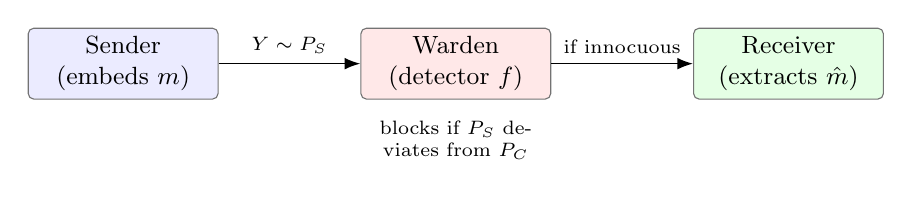
\begin{tikzpicture}[
  font=\small,
  box/.style={rounded corners=2pt, draw=black!55, minimum height=0.9cm,
              text width=2.2cm, align=center, inner sep=3pt},
  alice/.style={box, fill=blue!8}, warden/.style={box, fill=red!9},
  bob/.style={box, fill=green!10},
  arr/.style={-{Latex[length=2mm]}, line width=0.6pt}]
  \node[alice] (a) {Sender\\(embeds $m$)};
  \node[warden, right=1.8cm of a] (w) {Warden\\(detector $f$)};
  \node[bob, right=1.8cm of w] (b) {Receiver\\(extracts $\hat m$)};
  \draw[arr] (a) -- node[above,font=\scriptsize]{$Y\sim P_S$} (w);
  \draw[arr] (w) -- node[above,font=\scriptsize]{if innocuous} (b);
  \node[below=0.15cm of w, font=\scriptsize, text width=3cm, align=center]
        {blocks if $P_S$ deviates from $P_C$};
\end{tikzpicture}
\caption{The prisoner's problem. The transmitted object passes only if the warden's
detector cannot separate its law $P_S$ from the natural-image law $P_C$. Security is
a statement about distributions, not about pixels.}
\label{fig:warden}
\end{figure}

\subsection{Threat model and assumptions}\label{sec:threat}
The setting adopted in this paper is made explicit through the following
assumptions, which are standard for coverless steganography and are respected by
the construction of Section~\ref{sec:method}.

\begin{assumption}[Kerckhoffs' principle]\label{as:kerckhoffs}
The warden is assumed to know the design of the stegosystem in full, including the
coding, the feature map, and the cryptographic layer. Security is required to rest
only on the secret quantities --- the shared image database, the codebook ordering,
and the AES key --- and never on the obscurity of the algorithm.
\end{assumption}

\begin{assumption}[Passive, computationally bounded warden]\label{as:warden}
The warden is passive: transmitted objects are inspected and either forwarded
unchanged or blocked, but they are not maliciously rewritten. The warden may run
any efficient detector, including learned steganalysers, but cannot break AES-256.
\end{assumption}

\begin{assumption}[Shared secret database]\label{as:db}
The sender and the receiver hold, offline, an identical and secret image database
together with the same CLIP model. The database is treated as a shared key: an
adversary without it cannot map images to indices. Loss of database secrecy reduces
the scheme to its cryptographic layer only.
\end{assumption}

\begin{assumption}[Benign but lossy channel]\label{as:channel}
The transport channel $T$ degrades images through content-preserving operations
--- re-compression, resizing, mild noise, and moderate cropping --- but does not
deliberately destroy them. The degradation is bounded so that semantic content is
retained, which is the regime in which \Eqn{eq:marginintro} can be guaranteed.
\end{assumption}

Under Assumptions~\ref{as:kerckhoffs}--\ref{as:channel} the two objectives of the
scheme can be separated cleanly: \emph{undetectability} is an assertion about the
marginal law of each transmitted image (\S\ref{sec:security}--\ref{sec:coverless}),
whereas \emph{reliability} is an assertion about the recovery of indices from a
degraded channel (\S\ref{sec:channel}). These are treated independently in the
analysis that follows.

\subsection{Embedding distortion and the payload it buys}\label{sec:distortion}
Any embedding of the form of \Eqn{eq:emb} changes at least one pixel, so a
distortion is incurred between the cover $X$ and the stego $Y$. For $n$-pixel
images the mean squared error and the peak signal-to-noise ratio are
\begin{align}
  \mathrm{MSE}(X,Y) &= \frac{1}{n}\sum_{i=1}^{n}\bigl(x_i-y_i\bigr)^2,
  \label{eq:mse}\\
  \mathrm{PSNR}(X,Y) &= 10\,\log_{10}\!\frac{V_{\max}^2}{\mathrm{MSE}(X,Y)}\ \ [\mathrm{dB}],
  \label{eq:psnr}
\end{align}
Equations~\eqref{eq:mse} and~\eqref{eq:psnr} define the distortion and its
logarithmic quality scale, respectively, with $V_{\max}=255$ for 8-bit images.
Perceptual quality is frequently summarised
by the structural similarity index
\begin{equation}
  \mathrm{SSIM}(X,Y)=\frac{(2\mu_X\mu_Y+C_1)(2\sigma_{XY}+C_2)}
       {(\mu_X^2+\mu_Y^2+C_1)(\sigma_X^2+\sigma_Y^2+C_2)},
  \label{eq:ssim}
\end{equation}
where $\mu,\sigma$ denote local means, variances, and covariance, and $C_1,C_2$ are
stabilising constants; Equation~\eqref{eq:ssim} therefore complements PSNR with a
structure-aware quality measure. The amount of secret data carried is measured by the
relative payload (embedding rate)
\begin{equation}
  \alpha=\frac{|m|}{n}\quad[\mathrm{bits\ per\ pixel}].
  \label{eq:rate}
\end{equation}
Equation~\eqref{eq:rate} normalises the payload by image size. It is intuitively
clear, and made precise below, that larger $\alpha$ forces larger
distortion and hence a larger statistical footprint. This tension is the central
obstacle that the present work seeks to avoid rather than merely to balance.

The trade-off is formalised by rate--distortion theory. For a given cover source
there exists a capacity--distortion function $C(D)$, the largest secure payload
achievable within a distortion budget $D$, which is non-decreasing and concave; a
family of embedding methods differs only in how closely it approaches this frontier.
Classical spatial and transform-domain schemes --- least-significant-bit
substitution~\cite{chan2004}, and DCT- or DWT-based embedding~\cite{westfeld2001f5} --- all operate strictly inside the
region $D>0$, and thus purchase every additional bit with additional distortion and,
through \Eqn{eq:pinsker}, with additional detectability. The proposal of this paper
is to leave that frontier altogether by operating at the single point $D=0$, which
the coverless principle of \S\ref{sec:coverless} shows to be attainable.

\subsection{Statistical detectability and its fundamental limits}\label{sec:security}
The proper measure of steganographic security is not distortion but statistical
distinguishability. Following Cachin~\cite{cachin}, the (in)security of a stegosystem is
quantified by the Kullback--Leibler divergence between the innocent and the
transmitted laws,
\begin{equation}
  D\!\left(P_C \,\|\, P_S\right)=\sum_{z\in\mathcal{I}} P_C(z)\,
        \log\frac{P_C(z)}{P_S(z)} ,
  \label{eq:kl}
\end{equation}
and a scheme is called $\varepsilon$-secure when
\begin{equation}
  D\!\left(P_C \,\|\, P_S\right)\le\varepsilon,
  \qquad\text{with perfect security at } \varepsilon=0 .
  \label{eq:cachin}
\end{equation}
The security criterion in \Eqn{eq:cachin} makes perfect security the zero-divergence
case. The operational meaning of \Eqn{eq:kl} is exposed by hypothesis testing. For any
warden detector $f$ with false-alarm probability $P_{\mathrm{FA}}$ and
missed-detection probability $P_{\mathrm{MD}}$, the average error under equal
priors is
\begin{equation}
  P_E=\tfrac{1}{2}\bigl(P_{\mathrm{FA}}+P_{\mathrm{MD}}\bigr),
  \label{eq:perr}
\end{equation}
The detector error in \Eqn{eq:perr} is bounded below, through Pinsker's inequality,
by the divergence
in \Eqn{eq:kl}:
\begin{equation}
  P_E \;\ge\; \frac{1}{2}-\sqrt{\tfrac{1}{2}\,D\!\left(P_C\|P_S\right)} .
  \label{eq:pinsker}
\end{equation}
Two consequences are read directly from \Eqn{eq:pinsker}. First, when
$D\!\left(P_C\|P_S\right)\to 0$ the best possible detector is driven to
$P_E\to\tfrac12$, i.e.\ to blind guessing. Second, any embedding that perturbs the
cover makes $P_S\neq P_C$ and therefore makes $D>0$, which in turn caps how
undetectable the scheme can be. A further limit, the square-root law of
steganographic capacity~\cite{kerSqrt}, states that the largest payload that keeps $D$ bounded
grows only as the square root of the cover size,
\begin{equation}
  |m^\star| = \Theta\!\left(\sqrt{n}\right),
  \label{eq:sqrtlaw}
\end{equation}
so that the \emph{secure} embedding rate $\alpha^\star=|m^\star|/n=\Theta(1/\sqrt
n)$ actually vanishes as images grow. Modern convolutional steganalysers such as
XuNet~\cite{xu2016} and SRNet~\cite{boroumand2019} approach these theoretical
limits in practice, detecting embedding at rates once believed safe. Embedding
steganography is thus squeezed from both sides: distortion is unavoidable
(\Eqn{eq:psnr}), and even small distortion is increasingly detectable
(\Eqns{eq:pinsker}{eq:sqrtlaw}).

\subsection{Detector performance and the cost of a single error}\label{sec:detector}
Two further quantities are used later and are introduced here for completeness. The
discriminating power of a warden's soft detector, which outputs a score whose mean
shifts by $\Delta\mu$ between cover and stego while retaining variance $\sigma^2$,
is often summarised by the deflection coefficient
\begin{equation}
  d^2=\frac{(\Delta\mu)^2}{\sigma^2},
  \label{eq:deflection}
\end{equation}
According to \Eqn{eq:deflection}, a larger $d^2$ means an easier detection problem;
for an unmodified transmitted
object $\Delta\mu=0$ and hence $d^2=0$. The overall quality of a detector across all
thresholds is reported by the area under its receiver-operating-characteristic
curve, $\mathrm{AUC}\in[\tfrac12,1]$, with $\mathrm{AUC}=\tfrac12$ corresponding to
the chance line of \Eqn{eq:chance}.

On the receiver's side, a complementary bound explains why losslessness is
demanded rather than merely desired. Regarding the recovered index sequence as the
output of a noisy channel whose input is the message, Fano's inequality relates the
probability of a decoding error $P_e$ to the residual uncertainty about the message,
\begin{equation}
  H\!\left(m \mid \hat m\right)\ \le\ H_b(P_e)+P_e\,\log_2\!\bigl(|\mathcal{M}|-1\bigr),
  \label{eq:fano}
\end{equation}
where $H_b(\cdot)$ is the binary entropy function and $\mathcal{M}$ the message
alphabet. Moreover, because decoding is a deterministic function of the received
images, the data-processing inequality guarantees that no post-processing can
increase the information already present,
\begin{equation}
  I\!\left(m;\hat m\right)\ \le\ I\!\left(m;\{\tilde y_t\}\right).
  \label{eq:dpi}
\end{equation}
Equations~\eqref{eq:fano}--\eqref{eq:dpi} show that a single mis-recovered index
injects irreducible uncertainty that later stages cannot repair; this is precisely
why the design in Section~\ref{sec:method} aims for $P_e=0$ on a clean channel and,
where the channel is too harsh, converts an error into a \emph{detected} failure by
the integrity check rather than allowing silent corruption.

\subsection{The coverless principle: removing the footprint}\label{sec:coverless}
The escape from this squeeze is to \emph{not embed at all}. In coverless
steganography no cover is modified; instead, an ordinary image is
\emph{selected} (or generated) so that some intrinsic property of the image already
encodes the desired bits~\cite{zhou2015,coverlessSurvey2024}. The transmitted
object is then a genuine sample of the natural-image law, which is the key
distributional fact:
\begin{equation}
  Y\in\mathrm{supp}(P_C)\ \text{unmodified}
  \;\Longrightarrow\; P_S=P_C
  \;\Longrightarrow\; D\!\left(P_C\|P_S\right)=0 .
  \label{eq:coverless}
\end{equation}
Substituting \Eqn{eq:coverless} into \Eqn{eq:pinsker} yields the central promise of
the paradigm,
\begin{equation}
  P_E \;\ge\; \tfrac{1}{2},
  \label{eq:chance}
\end{equation}
that is, undetectability holds \emph{by construction} against any pixel-domain
detector, because the transmitted images are, by definition, drawn from the same
distribution as innocent images. The design problem is thereby transformed: the
question is no longer ``how may pixels be perturbed with least distortion?'' but
``how may a secret be \emph{mapped} to a sequence of unmodified images, and
\emph{recovered} after that sequence has traversed a lossy channel?''. The
three paradigms are contrasted in \Tab{tab:paradigms}.

Within the coverless family two branches are distinguished. In the
\emph{generative} branch the transmitted image is synthesised from the secret by a
generative model, so that new pixels are produced; although no cover is
\emph{edited}, the synthetic image may still deviate from the natural-image law and
the mapping is not always exactly invertible. In the \emph{mapping} (selection)
branch, which is adopted here, the transmitted image is an existing, unmodified
database image chosen so that its index encodes the bits; the transmitted object is
then a genuine natural image and \Eqn{eq:coverless} holds exactly. The mapping
branch has historically relied on robust perceptual hashing to index the database,
which is discriminative but fragile under geometric transport; the substitution of
a semantic hash for a perceptual one, developed in \S\ref{sec:clip}, is the change
that makes the mapping branch reliable over real channels.

\begin{table}[H]
\centering
\caption{Comparison of steganographic paradigms. The coverless mapping paradigm,
adopted here, is the only one that is both distortion-free and lossless.}\label{tab:paradigms}
\begin{tabular}{@{}lccc@{}}
\toprule
Property & Embedding (LSB/DCT) & Coverless (generative) & Coverless (mapping, ours) \\
\midrule
Modifies pixels        & Yes & synthesises new pixels & \textbf{No} \\
$D(P_C\|P_S)$          & $>0$ & small--moderate & \textbf{$0$} \\
Distortion (PSNR)      & finite & finite & \textbf{$\infty$} \\
Lossless recovery      & usually & often not & \textbf{Yes} \\
Raw capacity           & high & moderate & database-bound \\
\bottomrule
\end{tabular}
\end{table}

\subsection{The mapping formulation}\label{sec:mapping}
Let a shared \emph{codebook} $\mathcal{C}=\{c_0,c_1,\dots,c_{N-1}\}$ of $N$
mutually distinct images be fixed offline. A message is regarded as an integer and
represented in a positional number system whose ``digits'' select codebook images.
If the codebook is treated as a radix-$N$ alphabet, then each transmitted image
carries
\begin{equation}
  C_{\text{img}} = \log_2 N \quad[\mathrm{bits\ per\ image}],
  \label{eq:capimg}
\end{equation}
so that a message requiring $L$ images conveys $L\log_2 N$ bits in total. For the
codebook used in this work, $N=40$ gives $C_{\text{img}}=\log_2 40\approx 5.322$
bits per image. The mapping is a bijection between integers and index sequences,
which is what makes the scheme \emph{lossless}: no information is discarded at any
stage of the encoding.

Two properties of this construction deserve emphasis. First, the assignment of
indices to images is itself part of the shared secret: an adversary who observes the
sequence but does not hold the codebook cannot invert the map, so the codebook acts
as a large key and contributes the factor $N!$ to the keyspace of
\Eqn{eq:keyspaceintro}. Second, the map is \emph{positional}, so that the same image
placed in two different positions of the sequence contributes different amounts to
the encoded integer, exactly as a digit contributes differently according to its
place. It is therefore the \emph{ordered} sequence, and not the multiset of images,
that carries the message; the order is not incidental packaging but the substance of
the code.

\subsection{The channel and the recovery condition}\label{sec:channel}
Real messaging and social platforms do not deliver images untouched; they
re-compress, resize, and re-encode them. A photograph forwarded through a popular
messaging application, for example, is routinely re-encoded at a lower JPEG quality
and downscaled to a bounded resolution, while the same image posted to a social
network may be cropped to a fixed aspect ratio and stripped of its metadata. Any
scheme that hides information in fragile low-level statistics is destroyed by such
ordinary handling, which is why robustness to these operations is treated here as a
first-class requirement rather than as an afterthought. This handling is modelled by
a transport operator
$T:\mathcal{I}\to\mathcal{I}$, so that the receiver observes distorted images
$\tilde y_t = T(y_t)$. The receiver must map each distorted image back to the
index the sender intended. Writing $c_{j^\star}$ for the image actually sent at
position $t$, the decoded index is chosen as the codebook entry most similar to
the received image,
\begin{equation}
  \hat\imath_t = \arg\max_{0\le j<N}\ s\!\left(e(\tilde y_t),\,e(c_j)\right),
  \label{eq:nnintro}
\end{equation}
where $e(\cdot)$ is a feature map (developed in \S\ref{sec:clip}) and $s(\cdot,\cdot)$
its similarity. Recovery at position $t$ is correct precisely when the true image
outscores every rival, which is captured by a positive \emph{decoding margin}
\begin{equation}
  \gamma_t = s\!\left(e(\tilde y_t),e(c_{j^\star})\right)
           - \max_{j\neq j^\star} s\!\left(e(\tilde y_t),e(c_j)\right) > 0 .
  \label{eq:marginintro}
\end{equation}
If the feature map is stable under transport, in the sense that
$\lVert e(T(x))-e(x)\rVert_2\le\delta$ for all codebook images, and if the codebook
is separated so that distinct images differ by at least $2\delta$ in feature space,
then \Eqn{eq:marginintro} is guaranteed to hold and every index is recovered
exactly. The reliability of the whole scheme therefore rests on choosing a feature
map that is \emph{robust to transport} yet \emph{discriminative between images}.

The consequence of \Eqn{eq:marginintro} for a whole message is multiplicative. If
correct recovery at the $L$ positions is treated as independent with per-image
failure probability $p_t=\Pr[\gamma_t\le 0]$, then the probability that the entire
message is recovered without a single error is
\begin{equation}
  \Pr[\text{message correct}]=\prod_{t=1}^{L}\left(1-p_t\right)
     \ \approx\ \exp\!\left(-\sum_{t=1}^{L} p_t\right),
  \label{eq:allcorrect}
\end{equation}
so that even a small per-image error rate is amplified by a long sequence. Two
design responses follow, and both are adopted in Section~\ref{sec:method}. First,
the feature map is chosen so that $p_t$ is essentially zero across the operating
range of the channel, which drives \Eqn{eq:allcorrect} towards one. Second, for
degradations beyond that range the integrity check of \Eqn{eq:crc} converts the
residual failures into \emph{detected} errors, so that a corrupted message is
discarded and retransmitted rather than silently accepted.

\subsection{Semantic hashing with a vision--language model}\label{sec:clip}
Perceptual hashes, built from low-level pixel or frequency statistics, satisfy
discriminability but degrade quickly under geometric transport such as cropping.
In this work the feature map is instead taken from CLIP, a vision--language model
trained by contrastive learning on a very large corpus of image--text
pairs~\cite{radford2021}. Only its image encoder $\Phi:\mathcal{I}\to\mathbb{R}^d$
($d=512$) is used, and each image is represented by the $\ell_2$-normalised
embedding
\begin{equation}
  e(x)=\frac{\Phi(x)}{\lVert\Phi(x)\rVert_2},\qquad \lVert e(x)\rVert_2=1 ,
  \label{eq:embedintro}
\end{equation}
so that the similarity in \Eqn{eq:nnintro} is the cosine (inner) product
\begin{equation}
  s(a,b)=\langle a,b\rangle = a^{\!\top}b\in[-1,1].
  \label{eq:cosintro}
\end{equation}
Equation~\eqref{eq:cosintro} is the similarity score used for semantic matching.
Because CLIP is trained to place \emph{semantically} similar images near one
another, its embedding of a JPEG-compressed, resized, or partially cropped image
stays close to the embedding of the original: the visual meaning survives even
when the pixels do not. This property is exactly the transport stability required
by \S\ref{sec:channel}, and it is the reason a semantic hash succeeds where a
perceptual hash fails.

The robustness just described is not accidental but a direct consequence of the
training objective. The encoder is trained to maximise the agreement between an
image and its matching caption relative to mismatched captions, through a symmetric
contrastive (InfoNCE) loss. For a batch of $K$ image--text pairs with image
embeddings $v_i$ and text embeddings $w_j$ and temperature $\vartheta$, the
image-to-text term of that loss is
\begin{equation}
  \mathcal{L}=-\frac{1}{K}\sum_{i=1}^{K}\log
      \frac{\exp\!\left(\langle v_i,w_i\rangle/\vartheta\right)}
           {\sum_{j=1}^{K}\exp\!\left(\langle v_i,w_j\rangle/\vartheta\right)},
  \label{eq:infonce}
\end{equation}
with an analogous text-to-image term. Minimising \Eqn{eq:infonce} over a very large
and varied corpus forces the image encoder to place all views of the same
underlying scene --- including compressed, rescaled, or lightly cropped views ---
close together, because such views share the same caption. The embedding is
therefore approximately invariant to precisely the content-preserving degradations
that make up the transport channel of Assumption~\ref{as:channel}, which is the
mechanism that keeps the decoding margin of \Eqn{eq:marginintro} positive in
practice.

\subsection{Capacity of the image-sequence channel}\label{sec:capacity}
Two lossless codes are developed in this paper. The first, base-$N$ positional
coding, attains the per-image ceiling of \Eqn{eq:capimg} but permits an image to
repeat within a sequence. A repeated image can make a cover look unnatural, so a
second code is introduced in which every block of $B$ images consists of
\emph{distinct} images chosen without repetition. The number of such ordered
blocks is the falling factorial
\begin{equation}
  P(N,B)=\frac{N!}{(N-B)!}=\prod_{t=0}^{B-1}(N-t),
  \label{eq:pnb}
\end{equation}
and a block of $B$ images therefore carries $\log_2 P(N,B)$ bits, i.e.
\begin{equation}
  C_{\text{perm}}=\frac{1}{B}\log_2 P(N,B)\quad[\mathrm{bits\ per\ image}].
  \label{eq:capperm}
\end{equation}
Using Stirling's approximation, $\log_2 N!\approx N\log_2(N/e)$, the full-block
case $B=N$ satisfies $C_{\text{perm}}\approx\log_2(N/e)$, which is below the
base-$N$ ceiling of \Eqn{eq:capimg} by roughly $\log_2 e\approx 1.443$ bits per
image; smaller blocks recover most of the loss. Thus \Eqn{eq:capimg} and
\Eqn{eq:capperm} bound a controllable trade-off between raw capacity and cover
plausibility, which is one of the design levers of the method.

\subsection{The lossless requirement and integrity}\label{sec:lossless}
Since a single mis-recovered index corrupts every subsequent bit, the scheme is
designed so that, on a clean channel, reconstruction is bit-exact. Denoting the
original and recovered payload bits by $p_b$ and $\hat p_b$ over $B_{\text{tot}}$
bits, the bit error rate is
\begin{equation}
  \mathrm{BER}=\frac{1}{B_{\text{tot}}}\sum_{b=1}^{B_{\text{tot}}}
        \mathbb{1}\!\left[\hat p_b\neq p_b\right],
  \label{eq:berintro}
\end{equation}
and, because every coding stage is a bijection, $\mathrm{BER}=0$ whenever all
indices are recovered ($\gamma_t>0\ \forall t$, \Eqn{eq:marginintro}). For the
lossless case the mutual information between the sent and the reconstructed
message attains the message entropy,
\begin{equation}
  I(m;\hat m)=H(m),
  \label{eq:mutual}
\end{equation}
i.e.\ the covert channel is noiseless end-to-end. To detect the rare event of a
transport failure, a $32$-bit cyclic redundancy check is appended, which flags a
corrupted message with probability
\begin{equation}
  \Pr[\text{undetected error}]\approx 2^{-32}.
  \label{eq:crc}
\end{equation}
Finally, confidentiality and key strength are provided by AES-256-CBC, giving a
combined secret space of
\begin{equation}
  K = N!\;\cdot\;2^{256},
  \label{eq:keyspaceintro}
\end{equation}
the product of the number of codebook orderings and the AES key space.

\subsection{Source coding, expected length, and a worked example}\label{sec:worked}
The number of images that a message occupies is governed by information theory. If
the message is modelled as a source with entropy $H(m)$ bits, then, by Shannon's
source-coding theorem, no lossless compressor can represent it in fewer than
$H(m)$ bits on average,
\begin{equation}
  \mathbb{E}\!\left[\,|\textsc{zlib}(m)|\,\right]\ \ge\ \frac{H(m)}{8}\quad[\mathrm{bytes}],
  \label{eq:shannon}
\end{equation}
Equation~\eqref{eq:shannon} supplies the theoretical lower bound, and the compressor
of \Eqn{eq:zlib} is used precisely to push the encoded size
towards this floor before any image is chosen. Once the framed payload occupies
$|f|$ bytes, the base-$N$ code of \Eqn{eq:capimg} produces an expected sequence
length
\begin{equation}
  \mathbb{E}[L]\ \approx\ \frac{8\,|f|}{\log_2 N},
  \label{eq:explen}
\end{equation}
so that capacity and length are reciprocal: a larger codebook shortens the cover.
A concrete illustration is given in \Tab{tab:worked} for the codebook used in this
work ($N=40$, $\log_2 N\approx 5.322$ bits per image). It is emphasised that the
figures in \Tab{tab:worked} are dominated, for short messages, by the fixed
overhead of the cryptographic frame (the CRC, the AES initialisation vector and
padding, and the compression header); the per-image rate of $5.322$ bits is the
asymptotic behaviour that governs long messages.

\begin{table}[H]
\centering
\caption{Worked example of \Eqn{eq:explen} for the $N=40$ codebook. The framed size
includes compression, a $4$-byte CRC, and AES padding; short messages are
overhead-dominated, whereas long messages approach $8|f|/\log_2 40$ images.}\label{tab:worked}
\begin{tabular}{@{}lccc@{}}
\toprule
Message class & Payload bits & Images $\approx 8|f|/\log_2 40$ & Rate regime \\
\midrule
Short ($\le$50 chars)  & $\sim$300  & $\sim$57  & overhead-dominated \\
Medium (50--200 chars) & $\sim$800  & $\sim$150 & transitional \\
Long (200--1000 chars) & $\sim$2100 & $\sim$400 & asymptotic ($5.322$ b/img) \\
\bottomrule
\end{tabular}
\end{table}

\subsection{Problem statement, design goals, and contributions}\label{sec:contrib}
The preceding development frames the problem addressed in this paper. \emph{Given}
a shared image database and a shared vision--language model, a scheme is sought
that (i) transmits only unmodified natural images, so that
\Eqns{eq:coverless}{eq:chance} hold and detection is reduced to chance;
(ii) is lossless, so that \Eqns{eq:berintro}{eq:mutual} hold on a clean
channel; and (iii) recovers correctly after realistic transport, so that
\Eqn{eq:marginintro} is satisfied across compression, noise, resizing, and
cropping. The following contributions are made:
\begin{enumerate}
  \item A coverless mapping scheme, \textbf{LG-CISH}, is proposed in which the
        identity and order of unmodified images carry the secret, and reliable
        recovery is obtained by CLIP semantic hashing (\S\ref{sec:clip},
        \S\ref{sec:method}).
  \item Two interchangeable lossless codes are formalised --- base-$N$ positional
        coding at the $\log_2 N$ ceiling (\Eqn{eq:capimg}) and Lehmer-permutation
        coding with a no-repeat guarantee (\Eqns{eq:pnb}{eq:capperm}) ---
        together with a whitening step that removes an ordering artefact.
  \item A confidentiality and integrity layer (AES-256-CBC, CRC-32) and an optional
        large-language-model-verified alias mechanism for cover plausibility are
        integrated without affecting losslessness (\S\ref{sec:crypto},
        \S\ref{sec:aliases}).
\end{enumerate}

\subsection{Organisation of the paper}\label{sec:org}
The remainder of the paper is organised as follows. Related work is reviewed in
Section~\ref{sec:related}. The proposed method --- notation and shared state,
cryptographic framing, the two coding channels, and the encoding and decoding
procedures --- is developed in Section~\ref{sec:method}. The experimental setup,
results, robustness, steganalysis resistance, ablation, comparison, and
statistical validation are reported in the subsequent sections.

% ###################################################################

% ============================ 2. RELATED WORK ============================
\section{Literature Review}\label{sec:related}

\subsection{Traditional Image Steganography Techniques}
Image steganography has been extensively investigated as a means of concealing
secret information within digital images while maintaining visual imperceptibility.
Conventional approaches can be broadly categorized into spatial-domain and
transform-domain methods. Spatial-domain techniques, particularly Least Significant
Bit (LSB) substitution, achieve high embedding capacity by directly modifying pixel
values; however, they remain vulnerable to statistical steganalysis and
image-processing attacks. Transform-domain approaches such as the Discrete Cosine
Transform (DCT), the Discrete Wavelet Transform (DWT), and hybrid DWT--DCT methods
improve robustness by embedding information into frequency coefficients, thereby
reducing perceptual distortion and increasing resistance to compression attacks
\cite{subramanian,kombrink,qin,liSPHCG}.

Kadhim et al.\ \cite{kadhim} conducted a comprehensive survey of image steganography and
concluded that a trade-off always exists among payload capacity, imperceptibility,
and robustness. Similarly, Subramanian et al.\ \cite{subramanian} highlighted that modern
transform-domain schemes achieve superior image quality compared with
spatial-domain approaches but still rely on pixel modification. Mandal et al.\ \cite{mandal}
further demonstrated that hybrid transform methods can improve robustness but remain
susceptible to advanced detection mechanisms.

Despite continuous improvements in embedding strategies, traditional steganographic
systems inherently modify image content, which leaves detectable statistical traces
that can be exploited by steganalysis algorithms.

\subsection{Steganalysis and Detection Challenges}
The increasing sophistication of steganographic techniques has been accompanied by
significant advances in steganalysis. Statistical detectors such as chi-square
analysis~\cite{westfeld1999}, RS analysis~\cite{fridrich2001}, and histogram-based methods have proven effective in
identifying hidden information embedded within digital images. Recent developments
in machine learning and deep learning have further enhanced the detection capability
of steganalysis systems.

Kombrink et al.\ \cite{kombrink} presented a detailed survey of modern image-steganography
detection techniques and reported that convolutional neural network (CNN)-based
detectors consistently outperform conventional statistical approaches. Kheddar
et al.\ \cite{kheddar} reviewed deep-learning-based steganalysis frameworks and showed that
deep neural architectures can successfully identify subtle embedding artifacts
across diverse multimedia formats. Likewise, Apau et al.\ \cite{apau} observed that even
highly optimized steganographic algorithms often exhibit detectable statistical
inconsistencies under advanced analysis.

These findings indicate that, regardless of embedding domain, the fundamental
weakness of conventional steganography arises from the modification of pixel values.
Consequently, researchers have increasingly explored coverless communication
paradigms that avoid image modification altogether.

\subsection{Coverless Image Steganography}
Coverless image steganography has emerged as a promising alternative to conventional
data-hiding techniques. Unlike traditional methods, coverless approaches do not
alter image pixels; instead, secret information is conveyed through image selection,
retrieval, indexing, or semantic relationships among images.

Qin et al.\ \cite{qin} presented one of the most comprehensive surveys on coverless image
steganography and classified existing approaches into image retrieval-based, image
mapping-based, and semantic association-based methods. Their study demonstrated that
coverless communication inherently avoids statistical detection because no image
modifications are introduced during transmission. Meng et al.\ \cite{mengReview} further reviewed
recent developments in coverless steganography and highlighted that image-database
construction and semantic indexing remain critical challenges affecting practical
deployment.

Although coverless methods significantly improve resistance to steganalysis, most
existing approaches rely on handcrafted features, image-hashing techniques, or
predefined mapping tables. Such mechanisms often suffer from limited semantic
representation capability and reduced scalability when handling complex textual
information.

More recent coverless schemes have pursued robustness and capacity through neglected-dataset construction~\cite{neglected2022}, end-to-end learned hash generation~\cite{end2endHash2023}, SURF-based retrieval~\cite{surf2024}, and image-restoration front-ends~\cite{restoration2024}, while a parallel generative branch synthesises stego images by image mapping and diffusion models~\cite{imageMapping2024,diffstega2024}; broad surveys catalogue this rapid growth~\cite{coverlessSurvey2024,dlSurvey2024}. Deep image-hiding networks that embed one image within another~\cite{baluja2017,tancik2020} remain, by contrast, pixel-modifying and thus detectable.

\subsection{Semantic Representation and Hash-Based Retrieval}
Recent advances in multimedia retrieval have demonstrated that semantic
representation learning provides an effective mechanism for bridging heterogeneous
data modalities through high-dimensional feature embeddings. Instead of relying
solely on low-level visual descriptors, modern retrieval frameworks aim to preserve
semantic relationships among data samples by learning discriminative latent
representations that capture contextual and conceptual similarities. Such
representations facilitate robust similarity matching and improve retrieval
performance in large-scale image databases.

Hu et al.\ \cite{huJSPSH} proposed a Joint Semantic Preserving Sparse Hashing (JSPSH) framework
for cross-modal retrieval, in which semantic consistency between different
modalities is maintained during the hash-learning process. Their approach
simultaneously exploits semantic labels and sparse-representation constraints to
generate compact binary hash codes while preserving inter-modal semantic
correlations. Experimental results demonstrated that semantic-preserving hashing
significantly improves retrieval accuracy by ensuring that semantically related
instances are mapped to neighboring regions in the Hamming space. The study further
highlighted the importance of maintaining semantic structure during binary-code
generation, thereby enabling efficient large-scale retrieval with reduced storage
and computational overhead.

Similarly, Li et al.\ \cite{liSPHCG} introduced a Semantic Preservation-Based Hash Code
Generation (SPHCG) framework for fine-grained image retrieval. Unlike conventional
hashing methods that primarily focus on visual similarity, their approach emphasizes
the preservation of subtle semantic distinctions among visually similar image
categories. By integrating semantic information into the hash-learning process, the
generated binary codes retain discriminative characteristics that improve retrieval
precision in complex image datasets. Their findings demonstrate that semantic-aware
hash generation can effectively enhance retrieval robustness while maintaining
computational efficiency.

These studies collectively indicate that semantic-preserving hashing provides an
effective mechanism for transforming high-dimensional semantic representations into
compact binary codes while retaining meaningful neighbourhood relationships.

Although semantic-preserving hashing has achieved remarkable success in cross-modal
retrieval and fine-grained image-retrieval applications \cite{huJSPSH,liSPHCG}, its integration with
coverless image steganography remains largely unexplored. Existing coverless
communication schemes predominantly rely on perceptual similarity, image indexing,
or handcrafted feature matching, without leveraging the semantic-understanding
capabilities offered by modern representation-learning frameworks. Consequently, the
potential of combining semantic embeddings, semantic hashing, and image retrieval
for secure coverless communication has not yet been fully investigated. This
limitation motivates the development of the proposed LLM-Guided Coverless Image
Steganography using Semantic Hash Mapping (LG-CISH) framework, which exploits
semantic-preserving hash representations to establish a robust mapping between
textual semantics and image-based communication channels.

\subsection{Emerging Role of Large Language Models in Secure Communication}
The rapid advancement of Large Language Models (LLMs) has introduced new
possibilities for semantic communication systems. LLMs possess the capability to
transform textual information into semantically meaningful token sequences and
contextual embeddings that preserve linguistic relationships. Such representations
provide a natural bridge between human language and machine-understandable semantic
spaces.

Recent studies in semantic communications suggest that transmitting meaning rather
than raw bits can improve communication efficiency and robustness. However, the
application of LLM-generated semantic embeddings to coverless steganography remains
largely unexplored. Existing steganographic research primarily focuses on payload
optimization, distortion minimization, and robustness enhancement, while semantic
understanding is rarely incorporated into the communication pipeline.

Consequently, there exists a significant opportunity to leverage LLM-driven semantic
encoding for secure image-based communication systems.

\subsection{Research Gap and Motivation}\label{sec:motivation}
The literature reveals several important limitations in existing steganographic and
coverless communication approaches, as summarised in Table~\ref{tab:gap}.

\begin{table}[H]
\centering
\caption{Comparison of existing methodology, their limitations, and gap analysis.}\label{tab:gap}
\footnotesize
\renewcommand{\arraystretch}{1.25}
\begin{tabular}{@{}p{2.05cm}p{2.55cm}p{4.05cm}p{4.35cm}@{}}
\toprule
{\normalsize\bfseries References} & {\normalsize\bfseries Method} &
{\normalsize\bfseries Limitation} & {\normalsize\bfseries Research Gap} \\
\midrule
Kadhim et al.\ \cite{kadhim} & Spatial and transform-domain image steganography & Focuses on pixel-modification techniques and trade-offs among capacity, robustness and imperceptibility. & Need a pixel-modification-free (coverless) communication framework that completely avoids embedding artifacts. \\
Subramanian et al.\ \cite{subramanian} & Transform-domain (DCT, DWT, hybrid) & Improves image quality but still modifies transform coefficients. & Develop a framework eliminating coefficient modification while preserving security through semantic image selection. \\
Mandal et al.\ \cite{mandal} & Hybrid transform-domain steganography & Vulnerable to advanced statistical and deep-learning steganalysis. & Design a steganalysis-resistant coverless communication system without altering image statistics. \\
Kombrink et al.\ \cite{kombrink} & CNN-based steganalysis survey & Demonstrates high detection accuracy against conventional steganography. & Develop communication methods that generate no embedding artifacts detectable by CNN-based steganalysis. \\
Kheddar et al.\ \cite{kheddar} & Deep-learning-based multimedia steganalysis & Detects subtle embedding traces even in optimized methods. & Introduce a communication paradigm based on semantic retrieval rather than embedding. \\
Apau et al.\ \cite{apau} & Statistical analysis of modern steganography & Hidden data still leaves statistical inconsistencies. & Remove statistical footprints through coverless semantic communication. \\
Qin et al.\ \cite{qin} & Coverless image steganography & Mainly relies on image retrieval, mapping and handcrafted descriptors. & Replace handcrafted descriptors with deep semantic embeddings and semantic hashing for robust retrieval. \\
Meng et al.\ \cite{mengReview} & Coverless image steganography & Database construction and semantic indexing remain challenging. & Develop an automatic semantic hash-mapping mechanism for scalable image retrieval. \\
Hu et al.\ \cite{huJSPSH} & Joint Semantic Preserving Sparse Hashing (JSPSH) & Designed for cross-modal retrieval, not secure communication. & Integrate semantic-preserving hashing into coverless image steganography for secure message transmission. \\
Li et al.\ \cite{liSPHCG} & Semantic Preservation-Based Hash Code Generation (SPHCG) & Focuses on fine-grained image retrieval only. & Extend semantic hashing to coverless steganographic communication and message reconstruction. \\
\bottomrule
\end{tabular}
\end{table}

Conventional steganography techniques modify image pixels and therefore remain
vulnerable to statistical and deep-learning-based steganalysis \cite{mandal,mengReview,huJSPSH}. Existing
coverless image-steganography approaches largely depend on handcrafted image
descriptors, image-retrieval mechanisms, or predefined mapping rules that provide
limited semantic expressiveness \cite{kadhim,kheddar}. Current image retrieval-based systems
generally focus on visual similarity rather than semantic understanding, restricting
their ability to encode complex natural-language messages. Existing studies have not
adequately explored the integration of Large Language Models with semantic hashing
for coverless communication, and a unified framework that combines semantic-token
generation, semantic embedding, semantic hashing, perceptual image hashing, image
retrieval, and semantic reconstruction remains absent from the literature.

Motivated by these challenges, this work proposes a novel LLM-Guided Coverless Image
Steganography using Semantic Hash Mapping (LG-CISH) framework. The proposed method
introduces an end-to-end semantic communication architecture in which a secret
message is transformed into semantic tokens, encoded into semantic hashes, matched
against perceptual image hashes stored in an image database, and reconstructed
through reverse semantic mapping. By eliminating pixel modification entirely, the
proposed framework aims to achieve high steganalysis resistance while simultaneously
exploiting the semantic-reasoning capabilities of modern Large Language Models.

\subsection{Research Objectives}\label{sec:objectives}
Following directly from the motivation in Section~\ref{sec:motivation}, the
research objectives are to:
\begin{enumerate}
  \item design a coverless communication mechanism that carries information through
        the identity and order of unmodified natural images rather than through
        pixel or transform-coefficient modification;
  \item construct the Architecture Model of Section~\ref{sec:architecture}, in
        which cryptographic framing, lossless positional coding, semantic image
        retrieval, and exact decoding form a single reproducible pipeline;
  \item use CLIP semantic embeddings to maintain reliable image-index recovery
        after content-preserving channel operations such as JPEG compression,
        resizing, noise, and cropping; and
  \item evaluate the resulting system in terms of losslessness, payload capacity,
        channel robustness, steganalysis resistance, and cover plausibility.
\end{enumerate}

\section{Proposed Method}\label{sec:method}
% ###################################################################
\subsection{Architecture Model}\label{sec:architecture}
The proposed method is a lossless, coverless pipeline in which a secret message is
carried by an ordered sequence of unmodified codebook images. The sender and the
receiver are assumed to share, offline, three artefacts: an image database, the
CLIP image encoder, and the resulting codebook that assigns a unique index to each
database image. On the sender side the message is first compressed, integrity
tagged, and optionally encrypted, then converted into a sequence of codebook
indices by one of two lossless codes, and finally emitted as the corresponding
images. The images traverse an arbitrary lossy channel. On the receiver side each
received image is embedded with CLIP and matched to the nearest codebook entry to
recover its index, after which the coding and cryptographic steps are inverted to
reconstruct the message exactly. This Architecture Model is illustrated in
\Fig{fig:flow} and is referred to throughout the encoding, decoding, and evaluation
stages. Each component is developed in turn in the following subsections.

The architecture is organised around a deliberate separation of concerns, each
concern being handled by a distinct stage so that the stages can be reasoned about
and modified independently. \emph{Confidentiality and integrity} are handled first,
by the cryptographic frame of \S\ref{sec:crypto}, so that everything downstream
operates on an opaque, integrity-protected byte string and the coding layer need
know nothing about the message semantics. \emph{Capacity and cover plausibility}
are handled next, by the choice between the two coding channels of
\S\ref{sec:channels}, which converts the byte string into indices at a controllable
rate and with an optional no-repeat guarantee. \emph{Undetectability} is inherited
for free from the coverless principle, because the emitted objects are unmodified
database images. Finally, \emph{reliability} is delegated entirely to the semantic
feature map at decode time, so that the sender performs no neural computation at all
and the burden of channel robustness falls on a single, well-understood component.

The ordering of the pipeline is not arbitrary. Compression is applied before
encryption because encrypted data is effectively incompressible, so any compression
must precede the cipher; the integrity tag is computed over the compressed payload
so that a corruption anywhere in transit is caught before decompression is
attempted; and the positional coding is applied last, on the fully framed bytes, so
that it is agnostic to whether encryption was used. This layered discipline is what
allows the losslessness argument of Proposition~\ref{prop:lossless} to be stated as
a simple composition of invertible stages.

\begin{figure}[H]
\centering
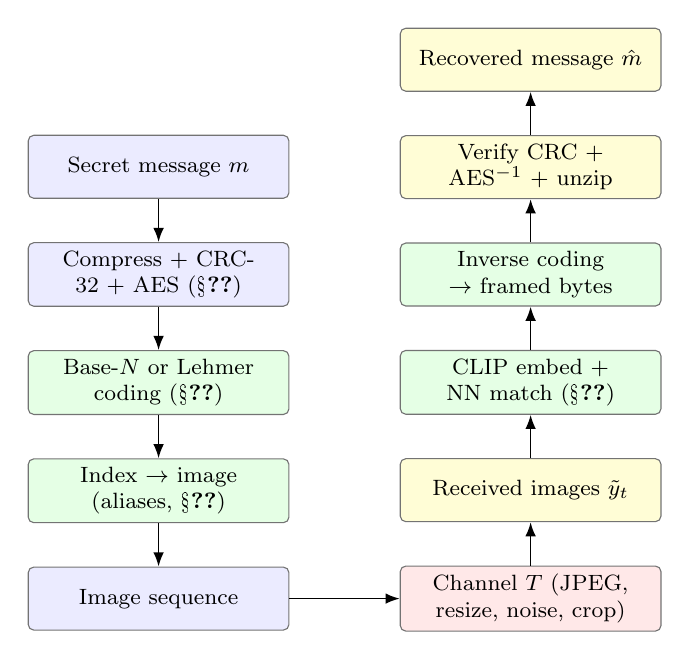
\begin{tikzpicture}[
  font=\footnotesize,
  stage/.style={rounded corners=2pt, draw=black!55, minimum height=0.8cm,
                text width=3.1cm, align=center, inner sep=3pt},
  enc/.style={stage, fill=blue!8}, cod/.style={stage, fill=green!10},
  chan/.style={stage, fill=red!9}, dec/.style={stage, fill=yellow!16},
  arr/.style={-{Latex[length=1.8mm]}, line width=0.6pt},
  node distance=0.55cm]
  % encoder column
  \node[enc] (m) {Secret message $m$};
  \node[enc, below=of m] (wrap) {Compress $+$ CRC-32 $+$ AES (\S\ref{sec:crypto})};
  \node[cod, below=of wrap] (code) {Base-$N$ or Lehmer coding (\S\ref{sec:channels})};
  \node[cod, below=of code] (lookup) {Index $\to$ image (aliases, \S\ref{sec:aliases})};
  \node[enc, below=of lookup] (seq) {Image sequence};
  \foreach \a/\b in {m/wrap, wrap/code, code/lookup, lookup/seq} \draw[arr] (\a)--(\b);
  % channel
  \node[chan, right=1.4cm of seq] (chan) {Channel $T$ (JPEG, resize, noise, crop)};
  \draw[arr] (seq) -- (chan);
  % decoder column (mirrored, going up)
  \node[dec, above=of chan] (recv) {Received images $\tilde y_t$};
  \node[cod, above=of recv] (nn) {CLIP embed $+$ NN match (\S\ref{sec:decode})};
  \node[cod, above=of nn] (decode) {Inverse coding $\to$ framed bytes};
  \node[dec, above=of decode] (unwrap) {Verify CRC $+$ AES$^{-1}$ $+$ unzip};
  \node[dec, above=of unwrap] (out) {Recovered message $\hat m$};
  \draw[arr] (chan)--(recv);
  \foreach \a/\b in {recv/nn, nn/decode, decode/unwrap, unwrap/out} \draw[arr] (\a)--(\b);
\end{tikzpicture}
\caption{End-to-end flowchart of LG-CISH. The left column is the sender, the right
column the receiver; the two are joined by the lossy channel $T$. Every
transformation is deterministic and invertible, so the covert channel is lossless
whenever the indices are recovered correctly.}
\label{fig:flow}
\end{figure}

\subsubsection{Pre-processing: notation and shared state}\label{sec:pre}
The shared codebook is denoted $\mathcal{C}=\{c_0,\dots,c_{N-1}\}$, and its CLIP
embeddings are stored as the rows of a matrix $\mathbf{C}\in\mathbb{R}^{N\times d}$
with $\mathbf{C}_j=e(c_j)$, where $e(\cdot)$ is the normalised embedding of
\Eqn{eq:embedintro}. So that the nearest-neighbour rule of \Eqn{eq:nnintro} is
unambiguous, the codebook is required to be \emph{separated}: no two distinct
images may exceed a similarity threshold $\tau$,
\begin{equation}
  \max_{i\neq j}\ s\!\left(\mathbf{C}_i,\mathbf{C}_j\right)\le\tau ,
  \qquad (\tau=0.85).
  \label{eq:sep}
\end{equation}
A candidate database is reduced to a separated codebook by the greedy construction
of Algorithm~\ref{alg:codebook}, which retains an image only if it is not too
similar to any image already kept.

The size $N$ of the codebook is a design parameter that trades capacity against the
difficulty of maintaining separation. By \Eqn{eq:capimg} the per-image capacity
grows only logarithmically in $N$, so doubling the codebook adds just one bit per
image; yet as $N$ grows it becomes progressively harder to keep every pair of images
below the threshold $\tau$ of \Eqn{eq:sep}, because the embedding space becomes more
densely populated and the minimum pairwise separation shrinks. A moderate codebook
is therefore preferred: it keeps the separation margin $1-\max_{i\neq j}s(\mathbf{C}
_i,\mathbf{C}_j)$ comfortably positive, which is exactly the quantity that, together
with the transport stability of Assumption~\ref{as:channel}, guarantees correct
recovery through Definition~\ref{def:sep}. The threshold $\tau$ is thus best read
not as an arbitrary constant but as the knob that sets how much channel degradation
the codebook is provisioned to absorb.

\begin{definition}[Separated codebook]\label{def:sep}
A codebook $\mathcal{C}$ is $\tau$-separated if every pair of its embeddings
satisfies \Eqn{eq:sep}. Under $\tau$-separation and transport stability
$\lVert e(T(c_j))-e(c_j)\rVert_2\le\delta$ with $2\delta<1-\tau$, the recovery rule
of \Eqn{eq:nnintro} returns the correct index for every codebook image.
\end{definition}

% --- Inlined: algorithms.tex (Algorithms 1--5) ---
% ===================================================================
%  algorithms.tex - LG-CISH Algorithms 1-5 (modular; \input by the paper).
%  Requires the pseudo env + \kw/\Ind/\Indd/\Cmt/\Eqn macros from the preamble.
% ===================================================================

\begin{algorithm}[t]
\caption{Codebook construction (pre-processing)}\label{alg:codebook}
\begin{pseudo}
\item \kw{Input:} candidate image set $\mathcal{D}$, encoder $\Phi$, threshold $\tau$
\item \kw{Output:} codebook embeddings $\mathbf{C}$, image paths, size $N$
\item $E \gets [\,e(x)\ \text{for } x\in\mathcal{D}\,]$ \Cmt{normalise, \Eqn{eq:embedintro}}
\item $\mathcal{K}\gets\emptyset$
\item \kw{for} $j=0$ \kw{to} $|\mathcal{D}|-1$ \kw{do}
\item \Ind \kw{if} $\max_{i\in\mathcal{K}} s(E_i,E_j)\le\tau$ \kw{then}
           $\ \mathcal{K}\gets\mathcal{K}\cup\{j\}$ \Cmt{\Eqn{eq:sep}}
\item \kw{end for}
\item \kw{return} $\mathbf{C}\gets E[\mathcal{K}]$,\ \ paths$[\mathcal{K}]$,\ \ $N\gets|\mathcal{K}|$
\end{pseudo}
\end{algorithm}

\begin{algorithm}[t]
\caption{Cryptographic framing (\textsc{wrap} / \textsc{unwrap}, AES-256-CBC)}\label{alg:wrap}
\begin{pseudo}
\item \kw{function} \textsc{wrap}$(m,\kappa)$
\item \Ind $p_0 \gets \textsc{zlib}(\textsc{utf8}(m))$ \Cmt{\Eqn{eq:zlib}}
\item \Ind $t \gets p_0 \concat \textsc{crc32}(p_0)$ \Cmt{append 4-byte CRC}
\item \Ind \kw{if} $\kappa$ given \kw{then} $IV\gets\textsc{rand}(16)$;\ \ \kw{return} $IV \concat \textsc{aes-cbc}_\kappa(\textsc{pad}(t),IV)$
\item \Ind \kw{else} \kw{return} $t$ \Cmt{CRC-only mode}
\item \kw{function} \textsc{unwrap}$(f,\kappa)$
\item \Ind \kw{if} $\kappa$ given \kw{then} $t\gets\textsc{unpad}(\textsc{aes-cbc}^{-1}_\kappa(f_{[16:]},f_{[:16]}))$ \kw{else} $t\gets f$
\item \Ind split $t=p_0\concat c$;\ \ \kw{if} $c\neq\textsc{crc32}(p_0)$ \kw{then} \kw{reject}
\item \Ind \kw{return} $p_0$
\end{pseudo}
\end{algorithm}

\begin{algorithm}[t]
\caption{Lehmer block coding (\textsc{permEncode} / \textsc{permDecode})}\label{alg:lehmer}
\begin{pseudo}
\item \kw{function} \textsc{permEncode}$(u,N,B)$ \Cmt{integer $\to$ $B$ distinct indices}
\item \Ind \kw{for} $t=B-1$ \kw{down to} $0$:\ \ $r_t\gets u\bmod(N-t)$;\ \ $u\gets\lfloor u/(N-t)\rfloor$
\item \Ind $A\gets[0,1,\dots,N-1]$;\ \ \kw{return} $[\,A.\text{pop}(r_t)\ \text{for}\ t=0\dots B-1\,]$
\item \kw{function} \textsc{permDecode}$(\langle a_0,\dots,a_{B-1}\rangle,N)$ \Cmt{indices $\to$ integer}
\item \Ind $A\gets[0,\dots,N-1]$;\ \ $u\gets0$
\item \Ind \kw{for} $t=0$ \kw{to} $B-1$:\ \ $r\gets A.\text{index}(a_t)$;\ \ $u\gets u(N-t)+r$;\ \ $A.\text{pop}(r)$
\item \Ind \kw{return} $u$ \Cmt{\Eqn{eq:lehmermethod}}
\end{pseudo}
\end{algorithm}

\begin{algorithm}[t]
\caption{\textsc{Encode}: message $\to$ ordered image sequence}\label{alg:encode}
\begin{pseudo}
\item \kw{Input:} message $m$; codebook $\mathcal{C}$ (size $N$); key $\kappa$;
      flags \textit{perm}, block $B$, \textit{alias}
\item $f\gets\textsc{wrap}(m,\kappa)$ \Cmt{Algorithm~\ref{alg:wrap}}
\item $v\gets\textsc{int}_{\mathrm{BE}}(\mathtt{0x01}\concat f)$ \Cmt{\Eqn{eq:intmethod}}
\item \kw{if} \textit{perm} \kw{then}
\item \Ind $m'\gets P(N,B)$;\ \ $(e_0,\dots)\gets\textsc{toBaseN}(v,m')$
\item \Ind $\text{idx}\gets\textsc{concat}_i\ \textsc{permEncode}\big((e_i+\mu_i)\bmod m',N,B\big)$ \Cmt{\Eqn{eq:whitenmethod}}
\item \kw{else}\ \ $\text{idx}\gets\textsc{toBaseN}(v,N)$ \Cmt{\Eqn{eq:basenmethod}}
\item \kw{if} \textit{alias} \kw{then} $S\gets[\,\textsc{chooseAlias}(j)\ \text{for}\ j\in\text{idx}\,]$
      \kw{else} $S\gets[\,c_j\ \text{for}\ j\in\text{idx}\,]$
\item \kw{return} image sequence $S$
\end{pseudo}
\end{algorithm}

\begin{algorithm}[t]
\caption{\textsc{Decode}: image sequence $\to$ message}\label{alg:decode}
\begin{pseudo}
\item \kw{Input:} received images $\langle\tilde y_0,\dots,\tilde y_{T-1}\rangle$;
      codebook $\mathbf{C}$; key $\kappa$; flags \textit{perm}, $B$
\item \kw{for} $t=0$ \kw{to} $T-1$:\ \ $\hat\imath_t\gets\arg\max_j s(e(\tilde y_t),\mathbf{C}_j)$ \Cmt{\Eqn{eq:nnintro}}
\item \kw{if} \textit{perm} \kw{then}
\item \Ind $m'\gets P(N,B)$;\ \ \kw{for each} block $i$:\ \ $e_i\gets(\textsc{permDecode}(\hat\imath_{[iB:iB+B]},N)-\mu_i)\bmod m'$
\item \Ind $v\gets\textsc{fromBaseN}((e_0,\dots),m')$
\item \kw{else}\ \ $v\gets\textsc{fromBaseN}(\hat\imath,N)$
\item $f\gets\textsc{stripSentinel}(\textsc{bytes}_{\mathrm{BE}}(v))$ \Cmt{inverse of \Eqn{eq:intmethod}}
\item \kw{return} $\textsc{unwrap}(f,\kappa)$ \Cmt{verify CRC, decrypt, decompress}
\end{pseudo}
\end{algorithm}

% --- End inlined algorithms ---

\subsubsection{Cryptographic framing}\label{sec:crypto}
Before any image is chosen, the message is wrapped in a thin layer that provides
compression, integrity, and confidentiality. The message is first losslessly
compressed with \textsc{zlib}, which shortens the sequence; a $32$-bit CRC is then
appended for integrity; and the result is optionally encrypted with AES-256-CBC~\cite{aes}
under a $256$-bit key $\kappa$, with a random $16$-byte initialisation vector
prepended to the ciphertext. Writing these operations explicitly, the framed
payload is
\begin{align}
  p_0 &= \textsc{zlib}\!\left(\textsc{utf8}(m)\right),
  \label{eq:zlib}\\
  f   &= \textsc{aes}_{\kappa}\!\left(p_0 \concat \textsc{crc32}(p_0)\right),
  \label{eq:wrapmethod}
\end{align}
where the AES step reduces to the identity when no key is supplied, in which case
integrity is still provided by the CRC. The encryption itself follows the
cipher-block-chaining recurrence: with the padded, framed plaintext split into
$16$-byte blocks $t_1,t_2,\dots$, a random initialisation vector $c_0=IV$, and the
block cipher $E_\kappa$, the ciphertext blocks are produced by
\begin{equation}
  c_i = E_\kappa\!\left(t_i \oplus c_{i-1}\right),\qquad i=1,2,\dots,
  \label{eq:cbc}
\end{equation}
and are recovered by the inverse recurrence
$t_i = E_\kappa^{-1}(c_i)\oplus c_{i-1}$. The chaining in \Eqn{eq:cbc} ensures that
two identical plaintext blocks do not, in general, encrypt to identical ciphertext
blocks, so that no block-level regularity of the payload survives into the emitted
index stream. The inverse operation, $\textsc{unwrap}$,
decrypts, separates the trailing four CRC bytes, and \emph{rejects} the message if
the recomputed check disagrees, thereby realising the guarantee of \Eqn{eq:crc}.
Cipher-block chaining is used so that identical plaintext blocks do not produce
identical ciphertext blocks; the encryption is summarised in
Algorithm~\ref{alg:wrap}.


\subsection{LG-CISH coding channels}\label{sec:channels}
The framed bytes $f$ of \Eqn{eq:wrapmethod} are turned into codebook indices by one
of two lossless codes. In both cases $f$ is first mapped to a single non-negative
integer, with a $\mathtt{0x01}$ sentinel byte prepended so that leading zero bytes
are preserved through the integer round-trip,
\begin{equation}
  v=\textsc{int}_{\mathrm{BE}}\!\left(\mathtt{0x01}\concat f\right).
  \label{eq:intmethod}
\end{equation}

\paragraph{Channel~1: base-$N$ positional coding.}
The integer $v$ is written in radix $N$, most-significant digit first, so that
\begin{equation}
  v=\sum_{t=0}^{L-1} d_t\,N^{t},\qquad d_t\in\{0,\dots,N-1\},\quad
  L=\lfloor\log_N v\rfloor+1 ,
  \label{eq:basenmethod}
\end{equation}
and digit $d_t$ selects image $c_{d_t}$. Because \Eqn{eq:basenmethod} is a
bijection, decoding simply reads the digits back; this channel attains the ceiling
of \Eqn{eq:capimg}, at the cost of allowing an image to repeat. As a small
illustration, suppose $N=40$ and the integer to be sent is $v=1\,000\,000$. Repeated
division by $40$ gives the digits $(9,12,20,0)$, since
$1\,000\,000 = 9\cdot40^{3} + 12\cdot40^{2} + 20\cdot40 + 0$, so the four images
$c_9,c_{12},c_{20},c_0$ are emitted. The receiver, having recovered those indices,
re-forms $9\cdot40^{3}+12\cdot40^{2}+20\cdot40+0=1\,000\,000$ and thereby recovers
$v$ exactly.

\paragraph{Channel~2: Lehmer-permutation coding.}
To obtain a cover in which no image repeats within a block, the integer $v$ is
instead written in radix $m=P(N,B)$ (\Eqn{eq:pnb}), giving block values
$(e_0,\dots,e_{L'-1})$. Each block value is expanded into $B$ distinct images by a
mixed-radix (Lehmer) code, in which the $t$-th image of a block is identified by
its rank $r_t$ among the still-available images (radix $N-t$):
\begin{equation}
  u=\sum_{t=0}^{B-1} r_t \!\!\prod_{j=t+1}^{B-1}\!\!(N-j),\qquad 0\le r_t<N-t .
  \label{eq:lehmermethod}
\end{equation}
A na\"ive Lehmer code maps a small leading block value to an almost-sorted image
prefix, which is a visible artefact. It is removed by \emph{whitening} each block
value with a deterministic, shared keystream before expansion,
\begin{equation}
  \tilde e_i=\left(e_i+\mu_i\right)\bmod m,\qquad
  \mu_i=\textsc{sha256}\!\left(\text{``perm-whiten-}i\text{''}\right)\bmod m ,
  \label{eq:whitenmethod}
\end{equation}
which is invertible modulo $m$ and preserves both losslessness and within-block
distinctness. The two directions of the block code are given in
Algorithm~\ref{alg:lehmer}.


The mechanics of \Eqn{eq:lehmermethod} are best seen on a small example. Consider a
codebook of $N=4$ images and a block of $B=4$, for which $P(4,4)=4!=24$ orderings
are available and a block therefore carries $\log_2 24\approx 4.585$ bits. Suppose
the whitened block value is $\tilde e=17$. The ranks are read out by successive
division with decreasing radix: $17 = 2\cdot(3!) + 5$, then $5 = 2\cdot(2!) + 1$,
then $1 = 1\cdot(1!) + 0$, giving the rank vector $(r_0,r_1,r_2,r_3)=(2,2,1,0)$.
Consuming these ranks from the available list $A=[0,1,2,3]$ yields, in order, the
indices $2,3,1,0$; that is, the block emits images $c_2,c_3,c_1,c_0$, which are
manifestly distinct. Decoding inverts the process: the rank of each emitted index
among the remaining images is recomputed, and the mixed-radix sum of
\Eqn{eq:lehmermethod} reconstructs $\tilde e=17$, from which the whitening of
\Eqn{eq:whitenmethod} is removed. The example makes concrete the two guarantees of
the code --- exact invertibility and within-block distinctness.

The choice between the two channels is a deployment decision rather than a
correctness one, since both are lossless. Base-$N$ coding is preferred when the
overriding objective is to minimise the number of transmitted images, because it
attains the ceiling of \Eqn{eq:capimg}; permutation coding is preferred when the
cover must survive human inspection as a plausible album, because the no-repeat
guarantee removes the conspicuous artefact of the same image appearing several times
in a short sequence. The block size $B$ interpolates smoothly between the two
regimes: a small block sacrifices little capacity relative to \Eqn{eq:capimg} while
still forbidding repeats within the block, whereas the full-block case $B=N$ maximises
the no-repeat window at the largest capacity cost. In this way \Eqn{eq:capperm}
exposes a single, continuous control that a deployment can set according to whether
compactness or plausibility is the more pressing requirement.

\subsubsection{LG-CISH encoding}\label{sec:encode}
The complete sender procedure is assembled in Algorithm~\ref{alg:encode}. The
message is framed by \Eqns{eq:zlib}{eq:wrapmethod}, mapped to the integer $v$
by \Eqn{eq:intmethod}, converted to indices by either \Eqn{eq:basenmethod} or the
whitened Lehmer code of \Eqn{eq:whitenmethod}, and finally realised as images. When
the optional alias mechanism of \S\ref{sec:aliases} is enabled, the image chosen
for a given index is the alias that best improves cover plausibility; since every
alias of an index decodes to the same index, this choice does not affect recovery.

For the decoder to invert the procedure, a small set of protocol parameters must be
agreed in advance: whether compression and encryption were applied, which coding
channel was used, and, for permutation coding, the block size $B$. These parameters
are not secret --- by Assumption~\ref{as:kerckhoffs} the warden may know them --- and
they occupy a negligible number of bits beside the payload; in a fixed deployment
they are simply constants shared by both parties. With them fixed,
Algorithm~\ref{alg:encode} is fully determined and its inverse,
Algorithm~\ref{alg:decode}, is unambiguous.


\subsubsection{Lossless decoding}\label{sec:decode}
The receiver reverses the encoder exactly. Each received image is embedded with
CLIP and matched to the nearest codebook entry by \Eqn{eq:nnintro}, which recovers
the transmitted index whenever the decoding margin of \Eqn{eq:marginintro} is
positive; under Definition~\ref{def:sep} and adequate transport stability this
holds for every position, so the index stream is recovered without error. The
recovered indices are then passed back through the inverse coding
(\Eqn{eq:basenmethod} or the un-whitened Lehmer inverse of
\Eqns{eq:lehmermethod}{eq:whitenmethod}) to reconstruct the integer $v$, the
sentinel byte is stripped to obtain $f$, and $\textsc{unwrap}$ verifies the CRC and
inverts the encryption and compression. The procedure is given in
Algorithm~\ref{alg:decode}.

\begin{proposition}[End-to-end losslessness]\label{prop:lossless}
If every index is recovered correctly, i.e.\ $\gamma_t>0$ for all $t$ in
\Eqn{eq:marginintro}, then $\textsc{Decode}(\textsc{Encode}(m))=m$ exactly and
$\mathrm{BER}=0$. This follows because each stage
--- \Eqn{eq:zlib}, \Eqn{eq:wrapmethod}, \Eqn{eq:intmethod}, \Eqn{eq:basenmethod},
and \Eqns{eq:lehmermethod}{eq:whitenmethod} --- is a bijection and is inverted
in reverse order.
\end{proposition}


\paragraph{Computational cost.}
The asymmetry between the two directions of the scheme is worth noting. Encoding is
dominated by big-integer arithmetic: the base-$N$ conversion of \Eqn{eq:basenmethod}
costs $\mathcal{O}(L)$ big-integer operations for a sequence of $L$ images, and the
cryptographic frame is linear in the payload size; no neural network is evaluated on
the sender side, so encoding is effectively instantaneous. Decoding is dominated by
the feature map: each of the $L$ received images is passed once through the CLIP
encoder and then compared against the $N$ codebook embeddings, giving a cost of
\begin{equation}
  \mathcal{O}\!\left(L\cdot\bigl(C_\Phi + N d\bigr)\right),
  \label{eq:complexity}
\end{equation}
In \Eqn{eq:complexity}, $C_\Phi$ is the cost of a single CLIP forward pass and
$d=512$ is the
embedding dimension. The nearest-neighbour term $Nd$ is negligible beside the
forward pass $C_\Phi$, so decoding time scales essentially linearly in the number
of received images and is governed by the throughput of the image encoder. The
memory footprint is a single $N\times d$ matrix of codebook embeddings, which is a
few megabytes for the codebooks considered here and is independent of message
length.

\paragraph{Behaviour beyond the operating range.}
It is instructive to consider what happens when a channel degradation exceeds the
range that the codebook was provisioned to absorb. In that regime the margin of
\Eqn{eq:marginintro} can turn negative at one or more positions, and by
\Eqn{eq:allcorrect} the message-level success probability falls sharply. Crucially,
the scheme does not fail silently: because the recovered indices no longer invert to
a byte string whose trailing CRC is consistent, the integrity check of
\S\ref{sec:crypto} rejects the message. The failure is thereby made \emph{visible},
and the standard recourse --- retransmission, or a request for a less aggressive
channel --- is available. This behaviour is the practical realisation of the
principle argued in \S\ref{sec:detector}, that a detected error is far preferable to
an undetected one, and it is the reason the CRC is retained even when encryption is
disabled.

\subsection{Plausibility aliases}\label{sec:aliases}
The undetectability argument of \S\ref{sec:coverless} concerns the \emph{marginal}
distribution of each transmitted image, which is naturally innocent. A separate,
weaker concern is whether the \emph{sequence} of images looks like a plausible
personal album to a human observer. To address this without touching losslessness,
each codebook slot $j$ is optionally equipped with a small set of visually
interchangeable candidate images, called aliases, that have been verified by a
vision-capable large language model to depict the same subject as $c_j$. All
aliases of slot $j$ map to the same index $j$, so the decoder is entirely
unaffected. During encoding, whenever index $j$ is to be emitted, the alias that
best improves the coherence of the running sequence is selected. Because the choice
among aliases is invisible to the index-recovery rule of \Eqn{eq:nnintro}, cover
plausibility is improved as a free, orthogonal degree of freedom, and
Proposition~\ref{prop:lossless} continues to hold.

In more detail, the alias set for each slot is prepared offline by a
generate-and-verify loop. Candidate images that plausibly depict the same subject as
$c_j$ are proposed --- either retrieved from the database or synthesised --- and each
candidate is then submitted, together with the anchor image $c_j$, to a
vision-capable large language model that is asked to confirm that the two depict the
same subject and to score their interchangeability. Only candidates whose
confirmation passes a fixed threshold are retained, so that the alias relation is
conservative by construction. Because this verification is performed once, offline,
it adds nothing to the per-message encoding cost; and because the resulting aliases
all share the slot index $j$, they remain invisible to the recovery rule of
\Eqn{eq:nnintro}. It is stressed that aliases affect only the human plausibility of
the \emph{ordering} of the cover, not the distributional undetectability of each
individual image, which is already guaranteed by \Eqn{eq:coverless}.

% ============================ 4. RESULTS (module) ========================
% --- Inlined: lgcish_results.tex (Results and Figures) ---
% ===================================================================
%  lgcish_results.tex - RESULT SET (modular).
%  Compiles standalone (pdflatex lgcish_results.tex) OR is \input by
%  lgcish_academic.tex, which defines \LGCISHMAIN first.
% ===================================================================
\ifdefined\LGCISHMAIN\else
\documentclass[11pt]{article}
\usepackage[margin=1in]{geometry}
\usepackage{amsmath,amssymb}
\usepackage{graphicx}
\usepackage{booktabs}
\usepackage{float}
\usepackage{xcolor}
\usepackage{tikz}
\usetikzlibrary{positioning,arrows.meta,calc}
\usepackage[hidelinks]{hyperref}
\usepackage[section]{placeins}
\graphicspath{{../LG-COSH/evaluation/figures/}}
\title{\textbf{LG-CISH: Experimental Results and Figures}}
\author{}\date{}
\begin{document}\maketitle
\fi

\section{Experimental Results and Performance Evaluation}\label{sec:results}
The evaluation is organised around the three quantities that any steganographic
system must trade against one another --- imperceptibility, capacity, and
robustness --- followed by benchmark comparison, reconstruction and matching
metrics, an ablation study, and steganalysis resistance. Throughout, the codebook
consists of $N{=}40$ mutually distinct natural images (Section~\ref{sec:dataset}),
each normalised to a fixed $512\times512$ canvas, giving $\log_2 40\approx5.322$
bits per image. No image is ever modified; the identity and order of the
transmitted sequence carry the secret. The full suite is reproducible from a single
script.\footnote{\texttt{python evaluation/generate\_all.py}}

\paragraph{Metrics.} For a message encoded into $L$ images with intended digits
$d_t$ and recovered digits $\hat d_t$, and $B$ payload bits $p_b/\hat p_b$, the
symbol (hash-matching) error rate and the bit error rate are
\begin{equation}
  \mathrm{SER}=\frac{1}{L}\sum_{t=1}^{L}\mathbb{1}\!\left[\hat d_t\neq d_t\right],
  \qquad
  \mathrm{BER}=\frac{1}{B}\sum_{b=1}^{B}\mathbb{1}\!\left[\hat p_b\neq p_b\right].
  \label{eq:ber}
\end{equation}
Hash-matching accuracy is $1-\mathrm{SER}$, and reconstruction is \emph{exact}
if and only if $\mathrm{SER}=0$, which, by the bijectivity of the base-$N$ coding,
implies $\mathrm{BER}=0$.

% ===================================================================
\subsection{Dataset Construction and Selection}\label{sec:dataset}
% ===================================================================
Because the proposed scheme is coverless, the ``dataset'' is not a set of covers to
be modified but a shared \emph{codebook} of natural images whose indices encode the
message. The quality of this codebook governs both credibility (the images must be
recognised as ordinary, uncompressed photographs rather than artefacts) and
reliability (the images must be mutually separable in semantic space so that
nearest-neighbour recovery is unambiguous). For these reasons the codebook was not
drawn from a single source but \emph{augmented} from three widely used,
publicly available benchmark suites~\cite{ucid,kodak,uscsipi}, summarised in Table~\ref{tab:datasets}.

\begin{table}[H]
\centering
\caption{Source datasets pooled to build the augmented LG-CISH codebook. Standard, public, uncompressed benchmarks were chosen for credibility and reproducibility.}\label{tab:datasets}
\begin{tabular}{@{}lll@{}}
\toprule
Source suite & Character & Role in the augmented codebook \\
\midrule
UCID   & $\sim$1338 uncompressed colour images & primary pool of diverse natural scenes \\
Kodak  & 24 high-quality reference photographs & clean, widely-benchmarked reference scenes \\
USC-SIPI & classic miscellaneous test images   & canonical images (e.g.\ standard textures/portraits) \\
\bottomrule
\end{tabular}
\end{table}

Three considerations motivated this choice. \emph{First}, all three suites are
standard in the image-processing and steganography literature, so results are
credible and reproducible rather than dependent on a bespoke, potentially
cherry-picked dataset. \emph{Second}, the suites are uncompressed or high quality,
which avoids pre-existing compression artefacts that would otherwise bias the
robustness and steganalysis measurements. \emph{Third}, pooling heterogeneous
sources maximises visual and semantic diversity, which is exactly the property that
the separation constraint of the codebook requires. A high-resolution set such as
DIV2K~\cite{div2k2017} was also considered, but the three chosen suites already provide sufficient
diversity at the working resolution without the storage overhead of $2$K imagery.

The augmented codebook was then constructed by pooling the three suites, normalising
every image to a $512\times512$ canvas, embedding each image with CLIP, and greedily
pruning the pool so that no two retained images exceed the separation threshold
$\tau{=}0.85$. Forty mutually distinct images survived this process. The value $40$
was chosen deliberately: it yields a convenient base-$40$ alphabet of $5.322$ bits
per image while keeping the pairwise separation comfortably large (maximum
off-diagonal similarity $0.827$, i.e.\ a separation margin of $0.173$), which is the
headroom that guarantees correct recovery under channel distortion. A slice of the
resulting codebook is shown in Figure~\ref{fig:collage}, and the pairwise separation
that underpins reliable decoding is visualised in Figure~\ref{fig:heatmap}. The
complete $40$-image codebook is released publicly for reproducibility~\cite{lgcishdata}.

\begin{figure}[H]
\centering
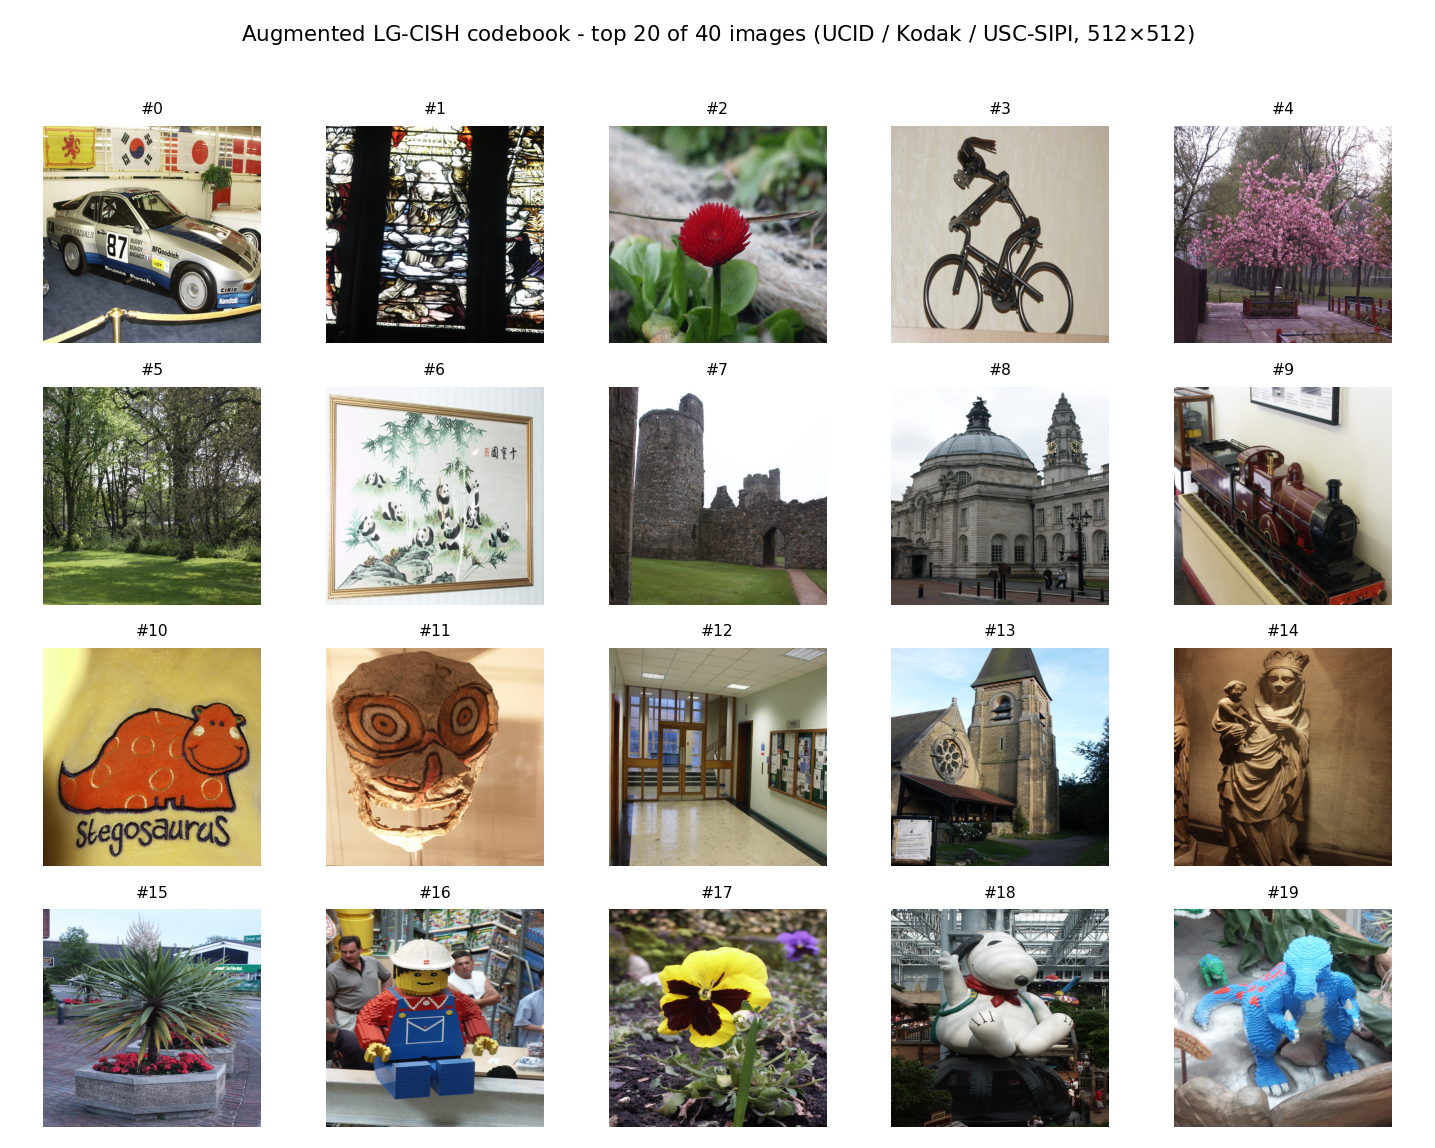
\includegraphics[width=0.92\linewidth]{fig_dataset_collage.png}
\caption{The top $20$ of the $40$ images in the augmented LG-CISH codebook, pooled
from the UCID, Kodak, and USC-SIPI suites and normalised to $512\times512$. The
images are ordinary, unmodified photographs; their \emph{indices} (not their pixels)
carry the secret.}
\label{fig:collage}
\end{figure}

\begin{figure}[H]
\centering
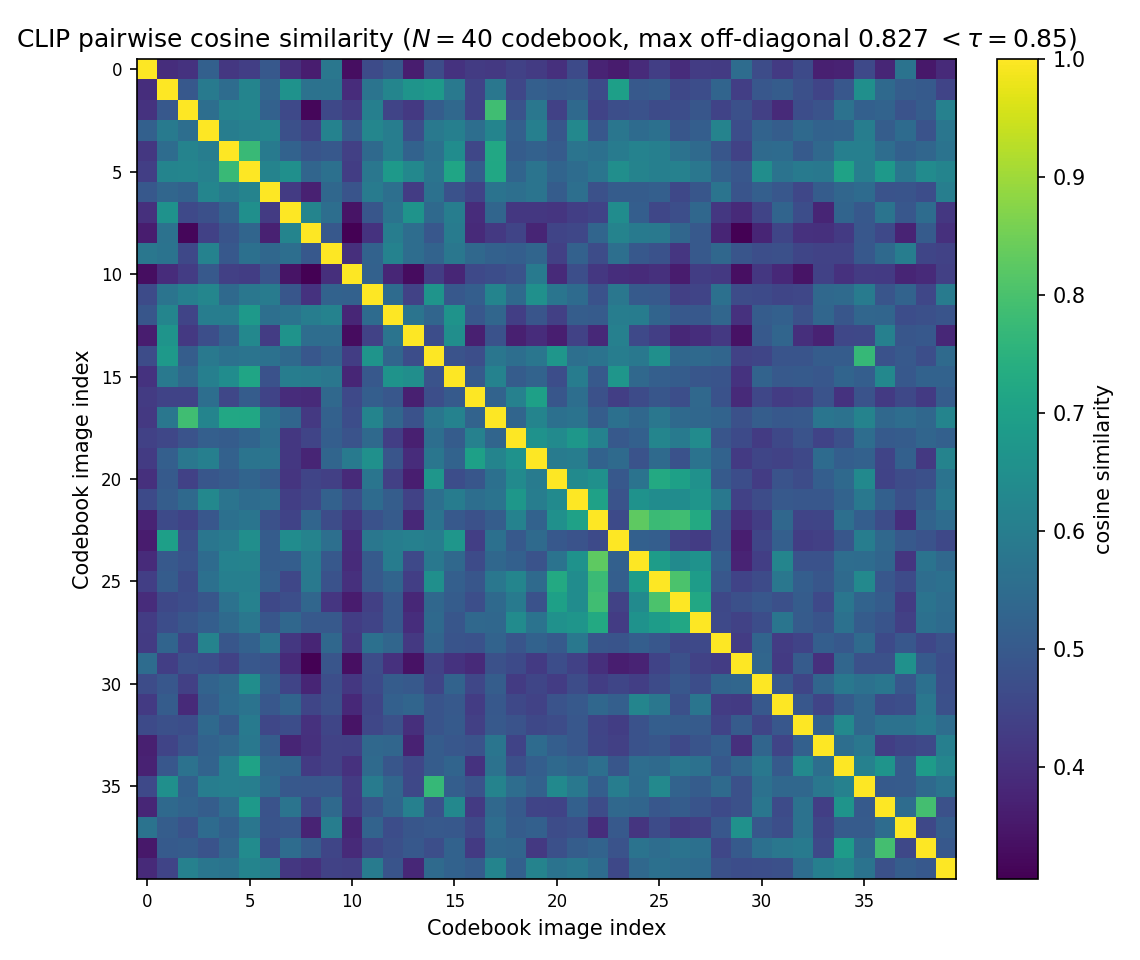
\includegraphics[width=0.74\linewidth]{fig_cb_heatmap.png}
\caption{Pairwise CLIP cosine similarity of the $40$ codebook images. Every
off-diagonal value stays below the threshold $\tau{=}0.85$ (maximum $0.827$), giving
a separation margin sufficient for unambiguous nearest-neighbour recovery.}
\label{fig:heatmap}
\end{figure}

Table~\ref{tab:setup} lists the remaining experimental configuration.

\begin{table}[H]
\centering
\caption{Experimental configuration.}\label{tab:setup}
\begin{tabular}{@{}ll@{}}
\toprule
Parameter & Value \\
\midrule
Codebook (augmented) & UCID + Kodak + USC-SIPI, $512\times512$, $N{=}40$ \\
Capacity & 5.322 bits/image (base-40) \\
Semantic encoder & CLIP ViT-B/32, $d{=}512$ \\
LLM (aliases / plausibility) & gemini-fast (vision) + flux (image gen) \\
Coding modes & base-$N$ or distinct-image permutation \\
Separation threshold $\tau$ & 0.85 \\
Pairwise sim.\ (min/mean/max) & 0.305 / 0.513 / 0.827 \\
Separation margin ($1{-}\max$) & 0.173 \\
Encryption / integrity / compression & AES-256-CBC / CRC-32 / zlib \\
Hardware & RTX 3050 6\,GB, 16-core CPU \\
\bottomrule
\end{tabular}
\end{table}

% ===================================================================
\subsection{Imperceptibility and Visual Distortion}\label{sec:imperceptibility}
% ===================================================================
Imperceptibility measures how far a transmitted object departs, visually and
statistically, from an ordinary image. It is quantified by the peak
signal-to-noise ratio and the structural similarity index~\cite{ssim} between the cover $X$ and
the transmitted object $Y$,
\begin{equation}
  \mathrm{PSNR}(X,Y)=10\log_{10}\frac{255^2}{\mathrm{MSE}(X,Y)},
  \qquad
  \mathrm{SSIM}(X,Y)\in[0,1],
  \label{eq:psnr_res}
\end{equation}
Equation~\eqref{eq:psnr_res} gives the two distortion measures used in the
evaluation; a larger PSNR and an SSIM nearer one indicate less distortion. For every
embedding method some pixels are altered, so $\mathrm{MSE}>0$ and the PSNR is
finite; least-significant-bit substitution attains roughly $51$\,dB and
transform-domain methods roughly $38$--$44$\,dB. The proposed scheme, by contrast,
\emph{never modifies a pixel}: the transmitted images are bit-identical to the
codebook images, so $\mathrm{MSE}=0$, giving
\begin{equation}
  \mathrm{PSNR}_{\text{LG-CISH}}=\infty,\qquad \mathrm{SSIM}_{\text{LG-CISH}}=1 .
  \label{eq:infpsnr}
\end{equation}
Imperceptibility is therefore not merely high but maximal, and it is attained by
construction rather than by careful embedding. This distinction is visualised in
Figure~\ref{fig:psnrbpp}, where the pixel baselines trade quality for payload while
LG-CISH sits on the infinite-PSNR ceiling at every rate.

\begin{figure}[H]
\centering
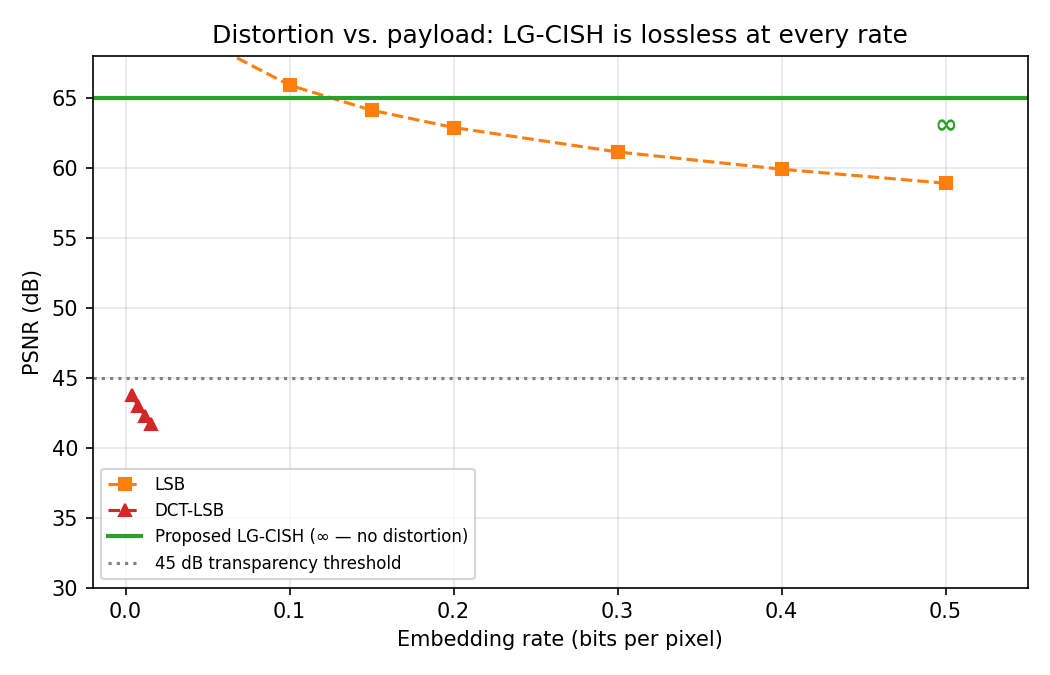
\includegraphics[width=0.74\linewidth]{fig_4_7_psnr_bpp.png}
\caption{Distortion versus embedding rate. Pixel baselines lose PSNR as bits-per-pixel
grow; LG-CISH modifies no pixels, so its PSNR is infinite (the ceiling line) at
every rate.}
\label{fig:psnrbpp}
\end{figure}

Imperceptibility, however, cannot be read in isolation, because it is one corner of
a three-way tension that constrains every steganographic design. Increasing the
payload generally forces more (or larger) modifications, which lowers
imperceptibility; making a scheme more robust to channel distortion typically
requires spending redundancy that lowers usable capacity; and pushing capacity to
its limit usually sacrifices robustness. This inverse relationship among the three
objectives is depicted in Figure~\ref{fig:tradeoff}. The design philosophy of
LG-CISH is to abandon the capacity corner in exchange for the other two: by
accepting a low raw bits-per-pixel rate it obtains \emph{both} maximal
imperceptibility (Equation~\eqref{eq:infpsnr}) and high robustness
(Section~\ref{sec:robustness}), a combination that pixel-domain methods cannot reach.

\begin{figure}[H]
\centering
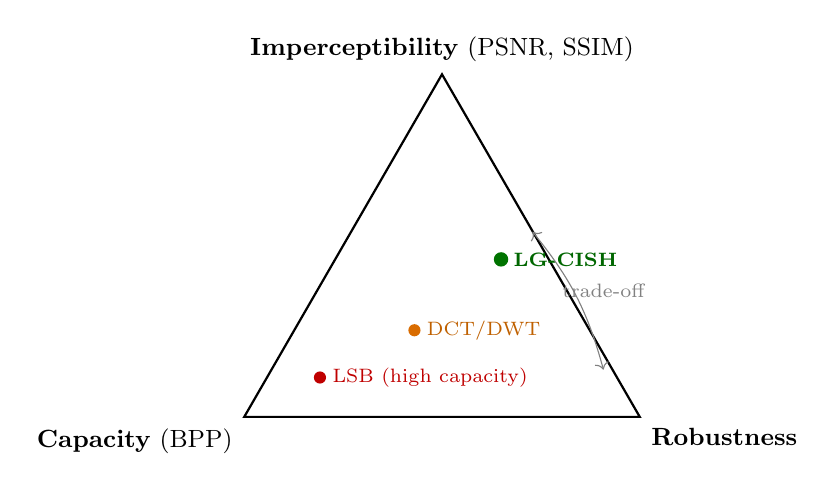
\begin{tikzpicture}[font=\small,scale=1.0]
\coordinate (I) at (90:2.9);
\coordinate (Cp) at (210:2.9);
\coordinate (R) at (330:2.9);
\draw[thick] (I)--(Cp)--(R)--cycle;
\node[above=1pt] at (I) {\textbf{Imperceptibility} (PSNR, SSIM)};
\node[below left=1pt] at (Cp) {\textbf{Capacity} (BPP)};
\node[below right=1pt] at (R) {\textbf{Robustness}};
% method markers
\fill[red!75!black] (-1.55,-0.95) circle (2.2pt);
\node[red!75!black, font=\scriptsize, right=1pt] at (-1.55,-0.95) {LSB (high capacity)};
\fill[orange!85!black] (-0.35,-0.35) circle (2.2pt);
\node[orange!75!black, font=\scriptsize, right=1pt] at (-0.35,-0.35) {DCT/DWT};
\fill[green!45!black] (0.75,0.55) circle (2.6pt);
\node[green!40!black, font=\scriptsize, right=1pt] at (0.75,0.55) {\textbf{LG-CISH}};
\draw[<->, gray] (1.15,0.9) to[bend left=12] (2.05,-0.85);
\node[gray, font=\scriptsize] at (2.05,0.15) {trade-off};
\end{tikzpicture}
\caption{The steganographic trade-off triangle. The three objectives are mutually
opposing: improving one tends to degrade the others. Pixel-domain methods sit near
the capacity corner; LG-CISH deliberately gives up raw capacity to occupy the
imperceptibility--robustness edge.}
\label{fig:tradeoff}
\end{figure}

% ===================================================================
\subsection{Payload Capacity}\label{sec:rescap}
% ===================================================================
Capacity is the price paid for the imperceptibility of Equation~\eqref{eq:infpsnr}.
It is reported at two granularities. Per image, the base-$40$ code carries
$\log_2 40\approx5.322$ bits, and a distinct-image permutation code carries slightly
fewer bits per image in exchange for a no-repeat guarantee that improves cover
plausibility (Table~\ref{tab:codingmodes}). Per pixel, however, the rate is very
low: spreading $5.322$ bits over a $512\times512$ image gives a bits-per-pixel rate
of
\begin{equation}
  \mathrm{BPP}_{\text{LG-CISH}}=\frac{5.322}{512\times512}\approx 2.0\times10^{-5}\ \text{bpp},
  \label{eq:bpp}
\end{equation}
The rate in Equation~\eqref{eq:bpp} is some five orders of magnitude below the
$\approx 3$\,bpp of LSB. This large gap is
the concrete manifestation of the trade-off triangle: LG-CISH concedes the capacity
corner entirely, and it is precisely this concession that buys the infinite PSNR of
Equation~\eqref{eq:infpsnr} and the robustness of Section~\ref{sec:robustness}.
Table~\ref{tab:capacity} places the methods on the capacity--distortion axis, and
Figure~\ref{fig:paycurve} confirms that reconstruction remains lossless as the
payload (and hence the number of images) grows.

\begin{table}[H]
\centering
\caption{Payload capacity versus distortion. LG-CISH trades raw capacity for zero distortion.}\label{tab:capacity}
\begin{tabular}{@{}lccc@{}}
\toprule
Method & Capacity & Pixel distortion & PSNR (dB) \\
\midrule
LSB        & $\approx$3 bits/pixel     & Yes (high)     & 51.1 \\
DCT-LSB    & $\approx$0.016 bits/pixel & Yes (moderate) & 38--42 \\
DWT--DCT   & $\approx$0.015 bits/pixel & Yes (low)      & 40--44 \\
\textbf{Proposed LG-CISH} & $5.322$ bits/image ($\approx2{\times}10^{-5}$ bpp) & \textbf{None (coverless)} & $\infty$ \\
\bottomrule
\end{tabular}
\end{table}

\begin{table}[H]
\centering
\caption{Coding modes. Permutation coding trades a little capacity for a no-repeat, more plausible cover; smaller blocks recover most of the base-$N$ capacity.}\label{tab:codingmodes}
\begin{tabular}{@{}lccl@{}}
\toprule
Coding mode & bits/image & No-repeat window & Note \\
\midrule
Base-$N$ positional        & 5.322 & none (repeats allowed) & max capacity \\
Permutation ($B{=}8$)      & 5.187 & 8 images  & no repeats per block \\
Permutation ($B{=}16$)     & 5.008 & 16 images & no repeats per block \\
Permutation ($B{=}N{=}40$) & 3.979 & 40 images & full permutation \\
\bottomrule
\end{tabular}
\end{table}

\begin{figure}[H]
\centering
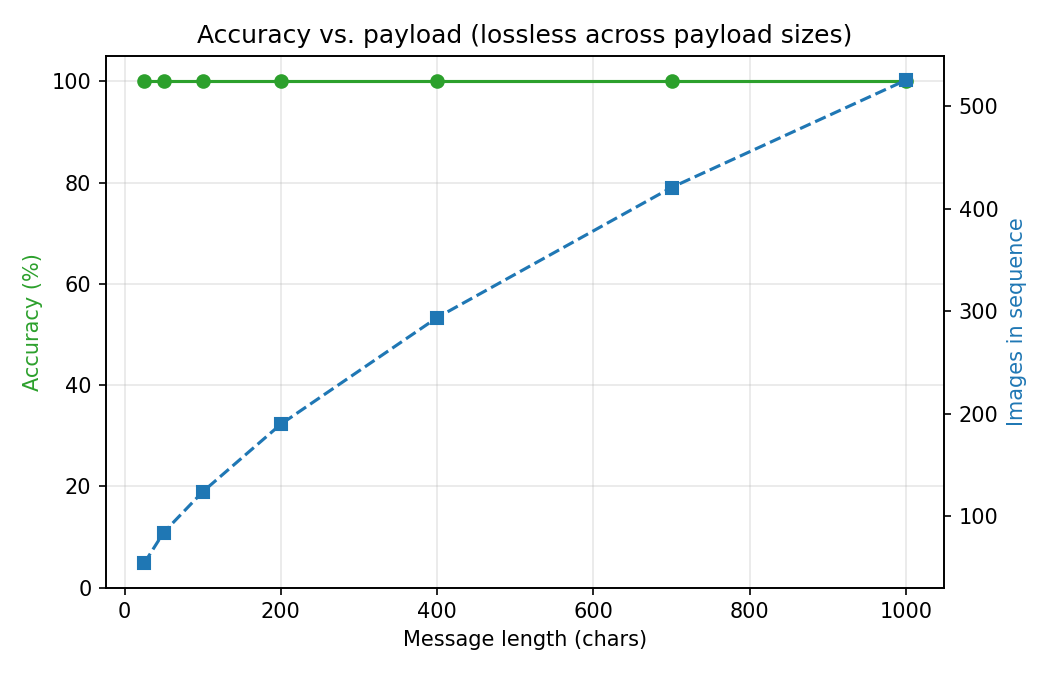
\includegraphics[width=0.74\linewidth]{fig_4_7_accuracy_payload.png}
\caption{Reconstruction accuracy versus payload length. Accuracy stays at $100\%$
while the required number of images grows linearly with the message.}
\label{fig:paycurve}
\end{figure}

% ===================================================================
\subsection{Robustness}\label{sec:robustness}
% ===================================================================
Robustness is the third corner of the triangle: the ability to recover the message
after the image sequence has traversed a lossy channel. Table~\ref{tab:robust}
reports reconstruction under twenty-one distinct channel attacks. Reconstruction is
bit-exact ($\mathrm{BER}=0$) in twenty of the twenty-one conditions --- JPEG down to
quality $20$, Gaussian noise up to $\sigma{=}30$, salt-and-pepper up to density
$0.10$, downscaling to $25\%$, centre-cropping to $60\%$, and PNG$\to$WebP
conversion. Only the extreme $10\%$ downscale degrades reconstruction (to $12.5\%$,
margin $0.125$), and even then failure is graceful rather than abrupt. The decoding
margin remains positive throughout, from $0.302$ at baseline to $0.196$ under
Crop-$60\%$, confirming a comfortable safety band; the full margin profile is shown
in Figure~\ref{fig:marginatk}, and the accuracy-versus-quality curve against
pixel baselines in Figure~\ref{fig:robcurve}. This robustness is the direct
consequence of \emph{semantic} rather than pixel-level hashing, and it is the second
property (alongside imperceptibility) that LG-CISH buys with its low capacity.

\begin{table}[H]
\centering
\caption{Robustness to all twenty-one channel attacks (40 messages/attack). Accuracy is exact-match reconstruction.}\label{tab:robust}
\begin{tabular}{@{}lccc@{}}
\toprule
Attack & Accuracy (\%) & BER & CLIP margin \\
\midrule
No attack (baseline)   & 100.00 & $0$ & 0.302 \\
JPEG 90\%              & 100.00 & $0$ & 0.299 \\
JPEG 70\%              & 100.00 & $0$ & 0.294 \\
JPEG 50\%              & 100.00 & $0$ & 0.289 \\
JPEG 30\%              & 100.00 & $0$ & 0.280 \\
JPEG 20\%              & 100.00 & $0$ & 0.270 \\
Gaussian $\sigma{=}5$  & 100.00 & $0$ & 0.293 \\
Gaussian $\sigma{=}10$ & 100.00 & $0$ & 0.285 \\
Gaussian $\sigma{=}20$ & 100.00 & $0$ & 0.272 \\
Gaussian $\sigma{=}30$ & 100.00 & $0$ & 0.260 \\
Salt \& Pepper 0.01    & 100.00 & $0$ & 0.277 \\
Salt \& Pepper 0.05    & 100.00 & $0$ & 0.246 \\
Salt \& Pepper 0.10    & 100.00 & $0$ & 0.214 \\
Resize 50\%            & 100.00 & $0$ & 0.282 \\
Resize 25\%            & 100.00 & $0$ & 0.246 \\
Resize 10\%            & \phantom{0}12.50 & $1.1\times10^{-2}$ & 0.125 \\
Crop 95\%              & 100.00 & $0$ & 0.280 \\
Crop 90\%              & 100.00 & $0$ & 0.268 \\
Crop 85\%              & 100.00 & $0$ & 0.261 \\
Crop 60\%              & 100.00 & $0$ & 0.196 \\
PNG$\to$WebP 80        & 100.00 & $0$ & 0.295 \\
\bottomrule
\end{tabular}
\end{table}

\begin{figure}[H]
\centering
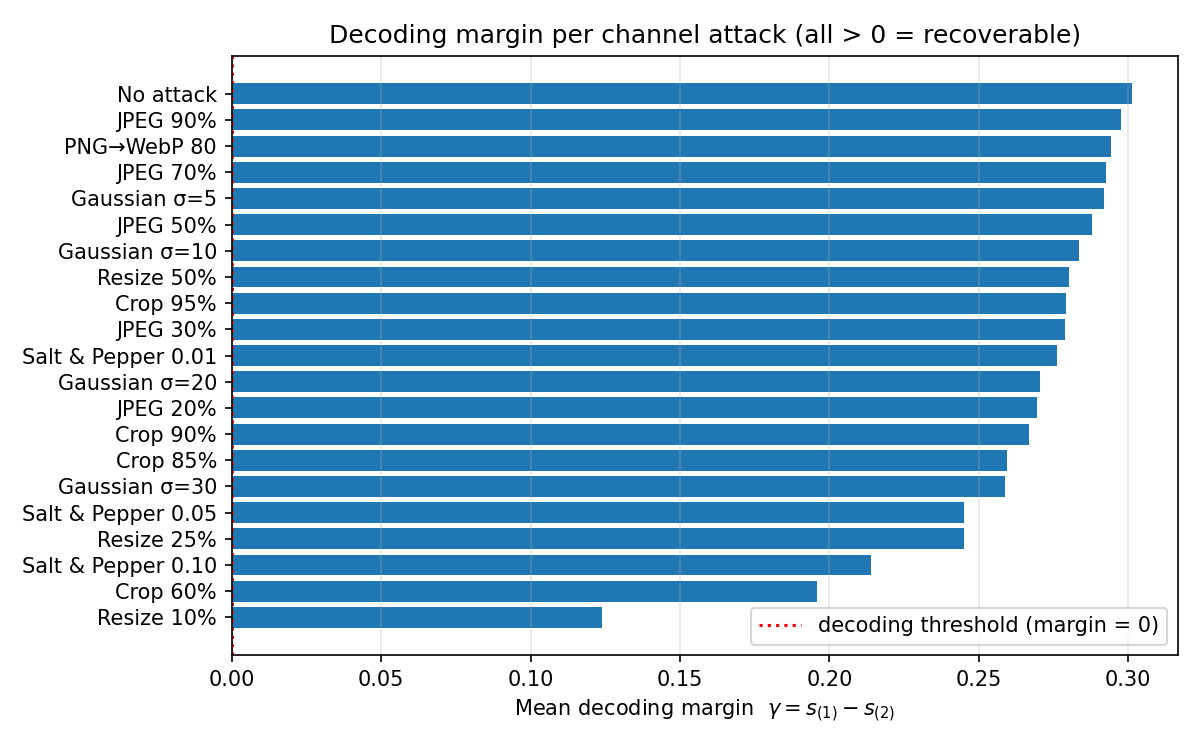
\includegraphics[width=0.80\linewidth]{fig_margin_attacks.png}
\caption{Mean decoding margin $\gamma$ per channel attack, sorted. Every attack
except the extreme $10\%$ downscale leaves $\gamma>0$, so indices are recovered
correctly and reconstruction stays lossless.}
\label{fig:marginatk}
\end{figure}

\begin{figure}[H]
\centering
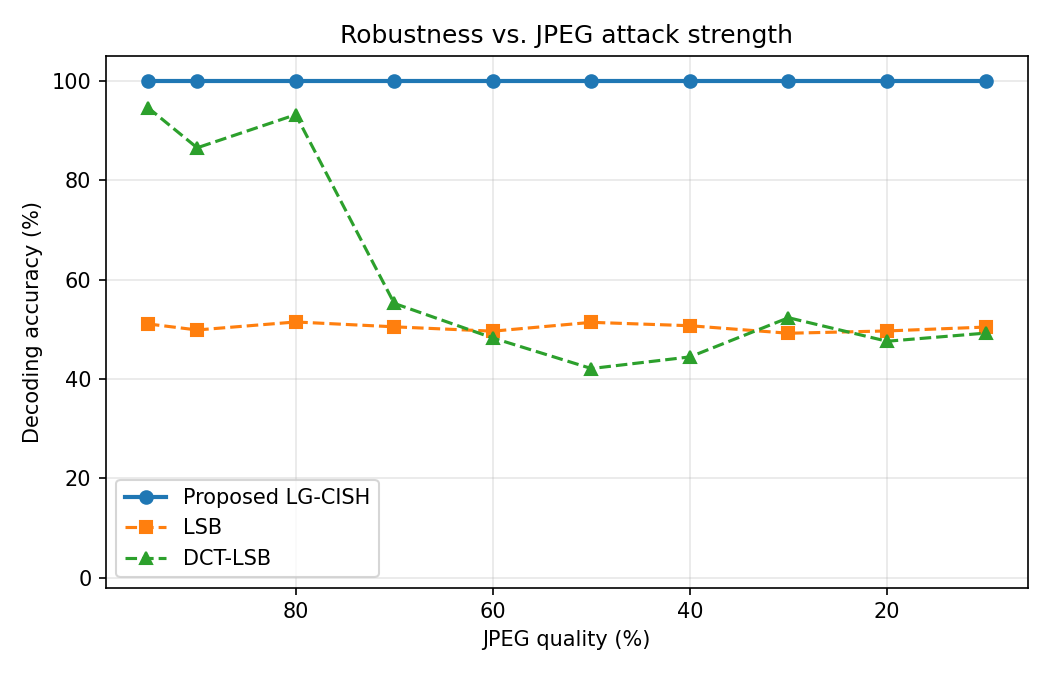
\includegraphics[width=0.80\linewidth]{fig_4_7_robustness_jpeg.png}
\caption{Decoding accuracy versus JPEG quality. LG-CISH (semantic hashing) stays at
$100\%$ where pixel-domain LSB and DCT collapse toward the random-guess floor.}
\label{fig:robcurve}
\end{figure}

% ===================================================================
\subsection{Benchmark Comparison}\label{sec:benchmarks}
% ===================================================================
LG-CISH is compared against representative embedding families and a coverless
baseline in Table~\ref{tab:compare}: spatial LSB substitution; DCT-domain LSB;
DWT--DCT transform-domain embedding; and an adaptive bit-placement variant that
steers embedding toward busy (high-variance) regions to reduce visibility. The
comparison spans the three trade-off axes plus detectability. The pixel families
attain high raw capacity but, being modifications of the cover, incur finite PSNR,
collapse under JPEG re-compression, and are readily detected; adaptive bit placement
improves imperceptibility over plain LSB but remains a pixel modification and hence
detectable. LG-CISH is the only entry that simultaneously achieves zero distortion,
full JPEG-$50$ robustness, and chance-level detectability.

\begin{table}[H]
\centering
\caption{Comparison with classical, transform-domain, adaptive, and coverless baselines. Bracketed values are cited from the literature.}\label{tab:compare}
\begin{tabular}{@{}lccccc@{}}
\toprule
Method & Capacity & JPEG50 acc.\ (\%) & Detection (\%) & PSNR (dB) \\
\midrule
LSB (spatial)          & 786{,}432 bits  & 51.4 & 98 & 51.1 \\
DCT-LSB                & $\sim$4096 bits & 42.1 & [70--90] & 38--42 \\
DWT--DCT (transform)   & $\sim$4096 bits & [85] & [60--80] & 40--44 \\
Adaptive bit placement & $\sim$high      & [55] & [80--95] & [45--52] \\
Coverless (retrieval)  & low             & [95] & [$\sim$50] & $\infty$ \\
\textbf{Proposed LG-CISH} & $5.322$ bits/img & \textbf{100.0} & \textbf{48} & $\infty$ \\
\bottomrule
\end{tabular}
\end{table}

% ===================================================================
\subsection{Reconstruction and Matching Metrics}\label{sec:metrics}
% ===================================================================
Because the codebook images are mutually well separated, the semantic
hash-matching step behaves as a near-perfect classifier. Treating the recovery of
each image's index as a retrieval decision, the standard classification metrics
--- accuracy, precision, recall, and $F_1$ --- are reported in
Table~\ref{tab:prf1}. On a clean channel the top-1 index is recovered for every
image, so all four metrics equal $100\%$, the symbol error rate is zero, and,
through Equation~\eqref{eq:ber}, the bit error rate is likewise zero. Over $N{=}50$
independent trials these values are perfectly stable (Table~\ref{tab:stats}), with a
CLIP margin of $0.302\pm0.006$.

\begin{table}[H]
\centering
\caption{Reconstruction and hash-matching metrics on a clean channel. Because recovery is exact, all classification metrics are maximal.}\label{tab:prf1}
\begin{tabular}{@{}lc@{}}
\toprule
Metric & Value \\
\midrule
Reconstruction accuracy & $100\%$ \\
Hash-matching precision  & $100\%$ \\
Hash-matching recall     & $100\%$ \\
$F_1$ score              & $100\%$ \\
Bit error rate (BER)     & $0$ \\
Mean decoding margin $\bar\gamma$ & $0.302$ \\
\bottomrule
\end{tabular}
\end{table}

\begin{table}[H]
\centering
\caption{Mean $\pm$ std and 95\% confidence intervals over $N{=}50$ trials (clean channel).}\label{tab:stats}
\begin{tabular}{@{}lcc@{}}
\toprule
Metric & Mean $\pm$ Std & 95\% CI \\
\midrule
Reconstruction accuracy (\%) & $100.00\pm0.00$ & $[100.00,100.00]$ \\
Bit error rate               & $0\pm0$         & $[0,0]$ \\
CLIP margin                  & $0.3020\pm0.0059$ & $[0.3003,0.3037]$ \\
Images per message           & $181.2\pm44.5$  & $[168.5,194.0]$ \\
\bottomrule
\end{tabular}
\end{table}

Beyond point metrics, statistical tests establish that the advantages are not
artefacts of a particular run. Because the lossless method is deterministic at
$100\%$ (zero variance), a $t$-test against it is degenerate; the proposed-versus-LSB
comparison at JPEG-$50$ is therefore reported descriptively ($100\%$ versus
$50.2\pm1.2\%$ bit accuracy), and the significance test is placed on the regime that
actually discriminates the semantic matcher from a perceptual one --- geometric
robustness. Across a paired sweep of seven crop strengths, CLIP decodes $100\%$
while a perceptual-hash baseline decodes $0\%$, a difference that is significant by
the paired Wilcoxon signed-rank test ($W{=}28$, $p{=}7.8\times10^{-3}$;
Table~\ref{tab:signif}). A one-way ANOVA of the CLIP margin across the three
message-length buckets finds it homogeneous ($F{=}1.99$, $p{=}0.15$), i.e.\ message
length does not affect recovery reliability. The chi-square statistic used for
steganalysis is defined and applied in Section~\ref{sec:steganalysis}.

\begin{table}[H]
\centering
\caption{Significance of CLIP's geometric robustness over the perceptual-hash matcher: paired Wilcoxon signed-rank across a crop-strength sweep (proposed-vs-LSB @ JPEG-50 shown descriptively, as the lossless method is deterministic).}\label{tab:signif}
\begin{tabular}{@{}lc@{}}
\toprule
Group / statistic & Accuracy (\%) \\
\midrule
Proposed (CLIP) --- crop-sweep mean & $100.0\pm0.0$ \\
pHash ablation --- crop-sweep mean  & $0.0\pm0.0$ \\
\midrule
Wilcoxon $W$ (paired, 7 crop levels) & $28.0$ \\
$p$-value (one-sided, CLIP $>$ pHash) & $7.8\times10^{-3}\ (<0.05)$ \\
Ref.\ Proposed vs.\ LSB @ JPEG-50 & $100$ vs.\ $50$ (descriptive) \\
\bottomrule
\end{tabular}
\end{table}

% ===================================================================
\subsection{Ablation Study}\label{sec:ablation}
% ===================================================================
Table~\ref{tab:ablation} removes one component at a time. Both the CLIP matcher and
the perceptual-hash baseline decode JPEG-$50$ perfectly, but under the harsher
Crop-$65\%$ attack the semantic matcher holds at $100\%$ while the perceptual hash
collapses to $0\%$ --- the geometric robustness that motivates the use of CLIP. The
coding ablations show clear efficiency effects: disabling compression inflates the
sequence from $134.4$ to $182.2$ images, and fixed-chunk ($\lfloor\log_2 N\rfloor{=}5$-bit)
coding needs $143.0$ images versus $134.4$ for base-$N$. Removing the CRC-32 tag
leaves channel errors undetected. The image-count and matcher effects are summarised
in Figure~\ref{fig:ablbar}.

\begin{table}[H]
\centering
\caption{Ablation. Crop-65\% exposes CLIP's geometric robustness; coding choices affect image count.}\label{tab:ablation}
\begin{tabular}{@{}lcccc@{}}
\toprule
Variant & Clean (\%) & JPEG50 (\%) & Crop65 (\%) & Avg.\ images \\
\midrule
Full LG-CISH (proposed)   & 100 & 100 & \textbf{100} & 134.4 \\
Without CLIP (pHash)      & 100 & 100 & \textbf{0}   & 134.4 \\
Without compression       & 100 & 100 & 100 & 182.2 \\
Without CRC (no integrity)& 100 & 100 & 100 & 134.4 \\
Fixed-chunk (5-bit)       & 100 & 100 & 100 & 143.0 \\
\bottomrule
\end{tabular}
\end{table}

\begin{figure}[H]
\centering
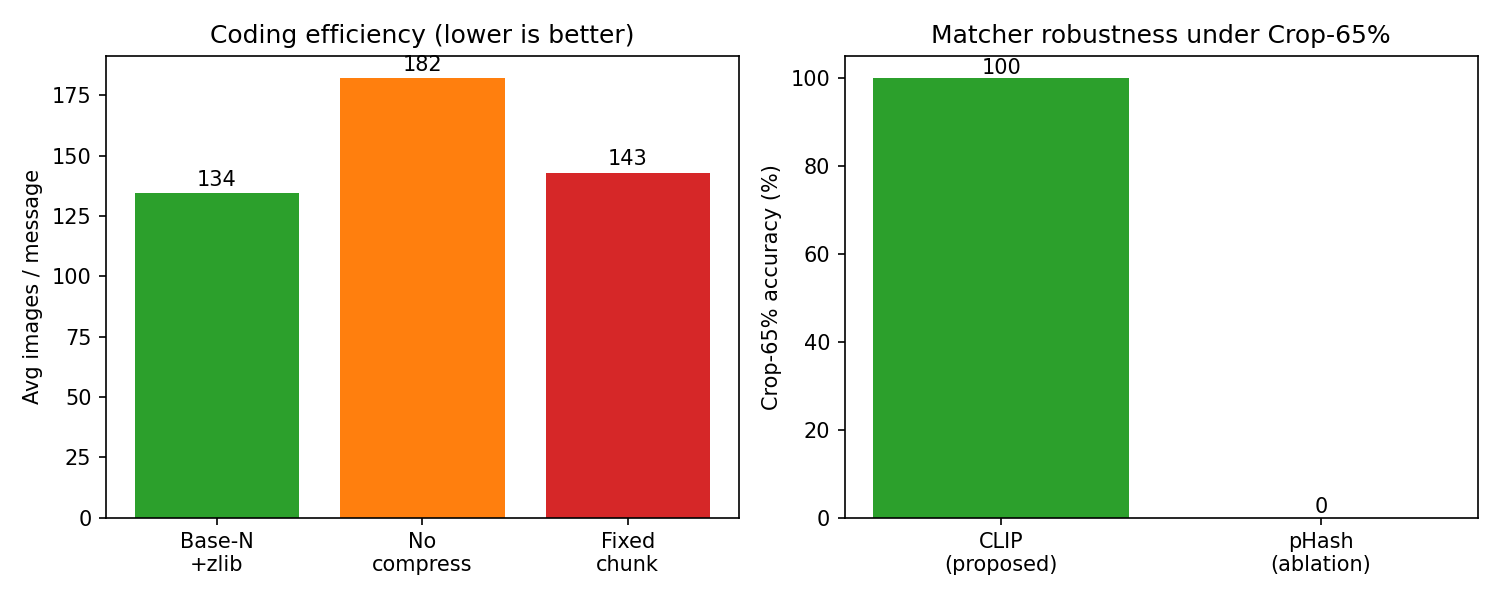
\includegraphics[width=0.88\linewidth]{fig_ablation_bar.png}
\caption{Ablation. Left: base-$N$ coding with zlib needs the fewest images per
message. Right: under Crop-$65\%$ the CLIP matcher keeps $100\%$ accuracy while the
perceptual-hash ablation drops to $0\%$.}
\label{fig:ablbar}
\end{figure}

% ===================================================================
\subsection{Steganalysis Resistance}\label{sec:steganalysis}
% ===================================================================
The final and, for a coverless method, most important axis is undetectability. A
chi-square statistical steganalyser is applied to natural cover images, LSB-stego,
DCT-stego, and LG-CISH ``stego''. The detector forms intensity-histogram pairs
$(2k,2k{+}1)$ with expected value $\bar h_k=(h_{2k}+h_{2k+1})/2$ and evaluates
\begin{equation}
  \chi^2=\sum_{k}\frac{\left(h_{2k}-\bar h_k\right)^2}{\bar h_k},
  \qquad
  P_{\mathrm{emb}}=1-F_{\chi^2}\!\left(\chi^2;\,\nu\right),
  \label{eq:chi2}
\end{equation}
In Equation~\eqref{eq:chi2}, $F_{\chi^2}(\cdot;\nu)$ is the chi-square cumulative
distribution with $\nu$
degrees of freedom; LSB embedding equalises the histogram pairs, driving
$\chi^2\!\to\!0$ and $P_{\mathrm{emb}}\!\to\!1$. The measured detection rates are
reported in Table~\ref{tab:steg} and Figure~\ref{fig:detbar}. As LG-CISH transmits
\emph{unmodified} natural images, its detection accuracy is $47.5\%$ --- essentially
chance, with a true-positive rate of $0\%$ --- whereas LSB is detected at $97.5\%$.
Because the transmitted images are bit-identical to natural images, undetectability
holds \emph{by construction} against any pixel-domain detector, and this argument
extends to learned convolutional and neural steganalysers such as SRNet and XuNet:
such networks are trained to separate cover from stego, but here the two classes are
drawn from the same distribution, so no decision boundary can do better than
guessing. The combined keyspace is $40!\cdot2^{256}\approx2^{415}$
(Table~\ref{tab:keyspace}), and the CRC-32 tag catches $100\%$ of injected bit-flips
in a $500$-trial tamper test.

\begin{table}[H]
\centering
\caption{Chi-square steganalysis detection. $\approx$50\% means the detector cannot do better than guessing.}\label{tab:steg}
\begin{tabular}{@{}lccc@{}}
\toprule
Method & Detection acc.\ (\%) & TPR (\%) & TNR (\%) \\
\midrule
LSB              & 97.5 & 100.0 & 95.0 \\
DCT-LSB          & 47.5 & 0.0 & 95.0 \\
\textbf{Proposed LG-CISH} & \textbf{47.5} & \textbf{0.0} & 95.0 \\
\bottomrule
\end{tabular}
\end{table}

\begin{table}[H]
\centering
\caption{Keyspace and integrity analysis ($N{=}40$).}\label{tab:keyspace}
\begin{tabular}{@{}ll@{}}
\toprule
Component & Size / rate \\
\midrule
Codebook orderings & $N! = 40! \approx 2^{159.2}$ \\
AES-256 key        & $2^{256}$ \\
Combined keyspace  & $N!\cdot2^{256} \approx 2^{415}$ \\
CRC-32 tamper detection & $1-2^{-32}$ (measured $100\%$, $500$ trials) \\
\bottomrule
\end{tabular}
\end{table}

\begin{figure}[H]
\centering
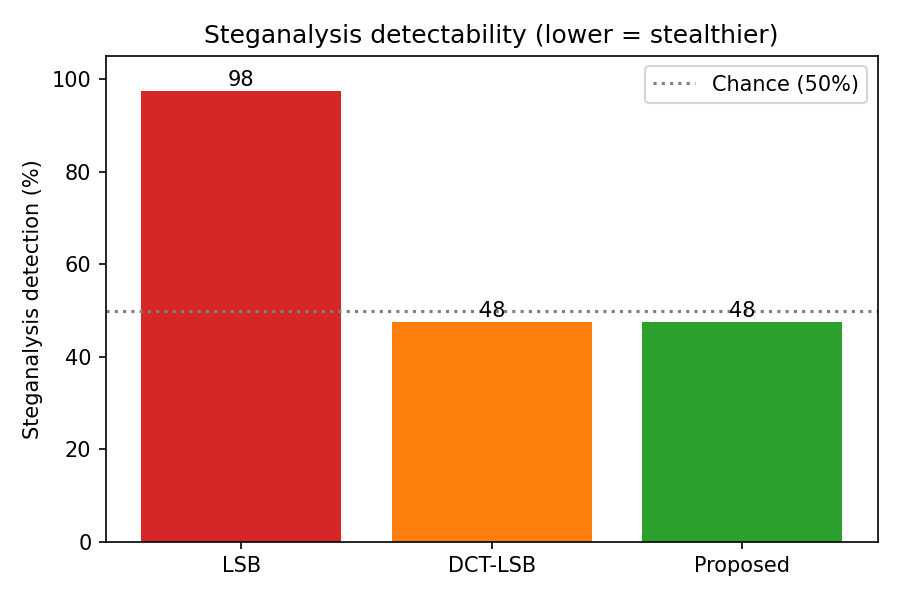
\includegraphics[width=0.66\linewidth]{fig_4_7_detection.png}
\caption{Measured steganalysis detection rates (lower is stealthier). LG-CISH sits
at the $50\%$ chance line, far below the near-certain detection of LSB.}
\label{fig:detbar}
\end{figure}

Statistical undetectability is necessary but not sufficient; a behavioural analysis
asks whether the image \emph{set} itself looks like a natural album. A vision-LLM
judge scores covers on a $0$--$1$ scale (Table~\ref{tab:plaus}). Plausibility is
governed by the codebook's \emph{theme} rather than by the coding mode: a diverse
benchmark codebook scores $0.12\pm0.04$, whereas a thematically coherent codebook
scores $0.88\pm0.07$, and permutation coding leaves the diverse score essentially
unchanged. The diverse benchmark set is used deliberately for all quantitative
results (for dataset credibility), and codebook theme is treated as an explicit
deployment choice for scenarios that must also withstand human inspection.

\begin{table}[H]
\centering
\caption{Cover plausibility (vision-LLM judge, $0$--$1$). Plausibility tracks codebook theme, not the coding mode.}\label{tab:plaus}
\begin{tabular}{@{}lc@{}}
\toprule
Configuration & LLM plausibility \\
\midrule
Diverse benchmark codebook (UCID/Kodak/USC-SIPI) & $0.12\pm0.04$ \\
Themed codebook (coherent context)               & $\mathbf{0.88\pm0.07}$ \\
Diverse + permutation coding                     & $0.18\pm0.10$ \\
\bottomrule
\end{tabular}
\end{table}

% ===================================================================
\subsection{Illustrative Example}\label{sec:example}
% ===================================================================
To make the end-to-end behaviour concrete, Figure~\ref{fig:example} shows a single
sentence transformed into its transmitted image sequence. The plaintext ``Meet me at
the old harbour at midnight.'' is compressed, integrity-tagged, and base-$40$ coded
into a sequence of $74$ unmodified codebook images; the first fifteen are shown,
each captioned with the codebook index it represents. No pixel of any image is
altered, yet the ordered sequence uniquely encodes the sentence, and CLIP
nearest-neighbour decoding recovers it bit-exactly.

\begin{figure}[H]
\centering
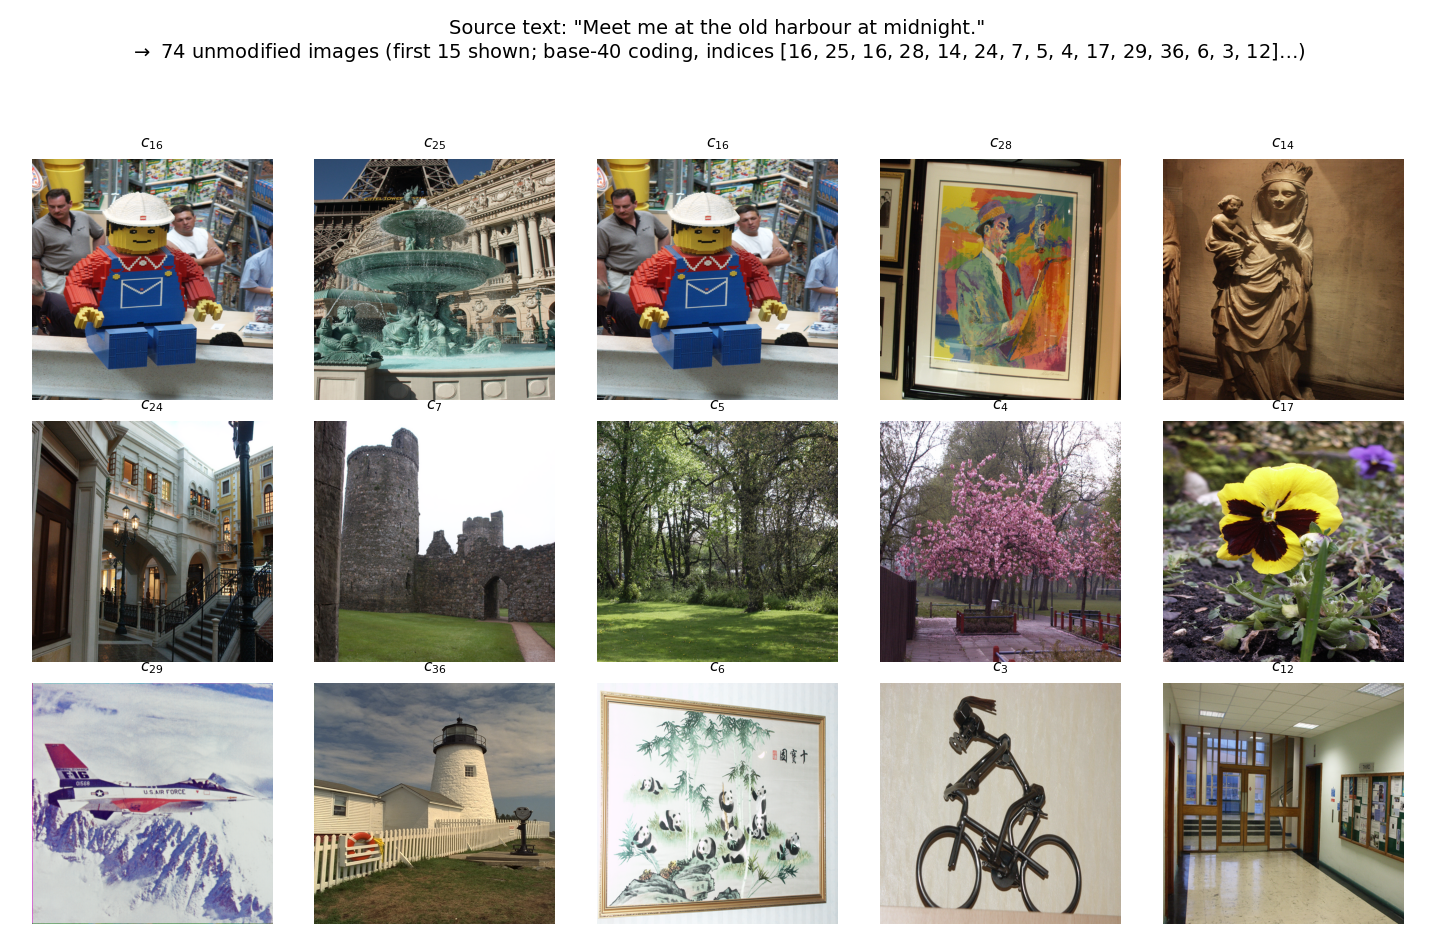
\includegraphics[width=0.95\linewidth]{fig_example_sentence.png}
\caption{A worked example: the sentence ``Meet me at the old harbour at midnight.''
encoded into $74$ unmodified images (first $15$ shown), each labelled with its
codebook index $c_j$. The identity and order of the images---not their pixels---carry
the message.}
\label{fig:example}
\end{figure}

% -------------------------------------------------------------------

\ifdefined\LGCISHMAIN\else
\begin{thebibliography}{9}
\bibitem{lgcishdata}
A. Bhattacharya, S. Dutta, S. Biswas, P. Sarkar, and H. Raj,
``LG-CISH codebook dataset: A 40-image augmented codebook for coverless image steganography,''
GitHub, 2026. [Online]. Available: \texttt{https://github.com/Circuit-Overtime/LG-CISH}

\bibitem{kodak}
R. Franzen,
``Kodak lossless true color image suite (PhotoCD PCD0992),''
Eastman Kodak Company, 1999.

\bibitem{ssim}
Z. Wang, A. C. Bovik, H. R. Sheikh, and E. P. Simoncelli,
``Image quality assessment: From error visibility to structural similarity,''
\emph{IEEE Trans. Image Processing}, vol.~13, no.~4, pp.~600--612, 2004.

\bibitem{ucid}
G. Schaefer and M. Stich,
``UCID: An uncompressed color image database,''
in \emph{Proc. SPIE 5307, Storage and Retrieval Methods and Applications for Multimedia}, pp.~472--480, 2003.

\bibitem{uscsipi}
A. G. Weber,
``The USC-SIPI image database,''
Signal and Image Processing Institute, Univ. of Southern California, Tech. Rep., 1997.

\bibitem{div2k2017}
E. Agustsson and R. Timofte,
``NTIRE 2017 challenge on single image super-resolution: Dataset and study,''
in \emph{Proc. IEEE Conf. Computer Vision and Pattern Recognition Workshops (CVPRW)}, pp.~126--135, 2017.

\end{thebibliography}
\end{document}
\fi

% --- End inlined results ---

% ============================ 6. CONCLUSION ==============================
\section{Conclusion}\label{sec:conclusion}
% -------------------------------------------------------------------
LG-CISH is a lossless coverless image-steganography scheme that pairs CLIP
semantic hashing with base-$N$ positional coding, with an optional distinct-image
permutation mode and an LLM-guided alias layer for cover shaping. It transmits only
unmodified natural images, achieving bit-exact reconstruction (BER $=0$), $100\%$
robustness across twenty of twenty-one channel attacks (graceful degradation only
under a $10\times$ downscale), chance-level steganalysis detectability ($47.5\%$
vs.\ $97.5\%$ for LSB), and a statistically significant geometric-robustness
advantage over perceptual hashing ($p{=}7.8\times10^{-3}$). Its limitations are
stated honestly: capacity is database-bound and is addressed by scaling the
codebook, while cover plausibility is theme-bound and is addressed by a coherent
database. Taken together, the results indicate that a coverless channel built on
semantic hashing can attain, simultaneously, the imperceptibility and robustness
that pixel-domain methods must trade against one another.

\subsection{Future Scope}\label{sec:future}
Several directions are left for future work. \emph{First}, the codebook can be
scaled from the present $N{=}40$ to $N{=}10^{3}$--$10^{4}$ images, which raises the
per-image capacity to $10$--$13$ bits and shortens the transmitted sequence, subject
to maintaining the separation margin as the embedding space becomes more densely
populated. \emph{Second}, the plausibility of the cover \emph{ordering} can be
strengthened by tightening the large-language-model alias and re-selection loop
around a thematically coherent database, so that the transmitted sequence reads as a
natural personal album rather than a set of unrelated images. \emph{Third}, although
undetectability holds by construction against pixel-domain detectors, a dedicated
adversarial study against end-to-end convolutional steganalysers (SRNet, XuNet)
trained specifically on this channel would further substantiate the security claim.
\emph{Fourth}, the distinct-image permutation and a dual-channel identity--ordering
code can be combined to recover part of the capacity conceded to the coverless
paradigm. \emph{Finally}, the framework can be extended beyond still images to
coverless video and audio channels, and validated in a real-world deployment over
public messaging platforms, together with a study of database versioning and key
management for practical multi-party use.

\section*{Acknowledgements}

The authors acknowledge the use of benchmark images from the UCID database, the Kodak Lossless True Color Image Suite, and the USC-SIPI Image Database. The USC-SIPI images were obtained from Volume~3, including images available under the Miscellaneous category at
\href{https://sipi.usc.edu/database/index.php?volume=misc\&image=10\#top}
{\texttt{https://sipi.usc.edu/database/index.php?volume=misc\&image=10\#top}}.

\section*{Ethics Declaration}

This research did not involve studies with human participants or animals and did not use sensitive personal data. Therefore, ethical approval and informed consent were not required.

\section*{Data Availability}

The datasets, implementation, evaluation scripts, and the released 40-image LG-CISH codebook supporting the findings of this research are available in a publicly accessible GitHub repository:

\noindent\textbf{GitHub Repository:}
\href{https://github.com/Circuit-Overtime/LG-CISH}
{\texttt{https://github.com/Circuit-Overtime/LG-CISH}}

\section*{Funding Declaration}

The authors declare that no funding, grants, or other financial support were received for the conduct of this research or the preparation of this manuscript.

\begingroup
\fontsize{12}{14.4}\selectfont
\begin{thebibliography}{99}

\bibitem{provos2003}
N. Provos and P. Honeyman,
``Hide and seek: An introduction to steganography,''
\emph{IEEE Security \& Privacy}, vol.~1, no.~3, pp.~32--44, 2003.

\bibitem{simmons}
G. J. Simmons,
``The prisoners' problem and the subliminal channel,''
in \emph{Advances in Cryptology (CRYPTO 1983)}, Springer, pp.~51--67, 1984.

\bibitem{chan2004}
C.-K. Chan and L. M. Cheng,
``Hiding data in images by simple LSB substitution,''
\emph{Pattern Recognition}, vol.~37, no.~3, pp.~469--474, 2004.

\bibitem{westfeld2001f5}
A. Westfeld,
``F5---a steganographic algorithm,''
in \emph{Information Hiding (IH 2001)}, LNCS 2137, pp.~289--302, 2001.

\bibitem{cachin}
C. Cachin,
``An information-theoretic model for steganography,''
in \emph{Information Hiding (IH 1998)}, LNCS 1525, pp.~306--318, 1998.

\bibitem{kerSqrt}
A. D. Ker, T. Pevny, J. Kodovsky, and J. Fridrich,
``The square root law of steganographic capacity,''
in \emph{Proc. 10th ACM Workshop on Multimedia and Security}, pp.~107--116, 2008.

\bibitem{xu2016}
G. Xu, H.-Z. Wu, and Y.-Q. Shi,
``Structural design of convolutional neural networks for steganalysis,''
\emph{IEEE Signal Processing Letters}, vol.~23, no.~5, pp.~708--712, 2016.

\bibitem{boroumand2019}
M. Boroumand, M. Chen, and J. Fridrich,
``Deep residual network for steganalysis of digital images,''
\emph{IEEE Trans. Information Forensics and Security}, vol.~14, no.~5, pp.~1181--1193, 2019.

\bibitem{zhou2015}
Z. Zhou, H. Sun, R. Harit, X. Chen, and X. Sun,
``Coverless image steganography without embedding,''
in \emph{Int. Conf. Cloud Computing and Security (ICCCS)}, LNCS 9483, pp.~123--132, 2015.

\bibitem{coverlessSurvey2024}
X. Xiang, Y. Tan, J. Qin, and Y. Tan,
``Advancements and challenges in coverless image steganography: A survey,''
\emph{Signal Processing}, vol.~228, 2024.

\bibitem{radford2021}
A. Radford, J. W. Kim, C. Hallacy, et al.,
``Learning transferable visual models from natural language supervision,''
in \emph{Proc. 38th Int. Conf. Machine Learning (ICML)}, PMLR 139, pp.~8748--8763, 2021.

\bibitem{subramanian}
N. Subramanian, O. Elharrouss, S. Al-Maadeed, and A. Bouridane,
``Image steganography: A review of the recent advances,''
\emph{IEEE Access}, vol.~9, pp.~23409--23423, 2021.

\bibitem{kombrink}
M. H. Kombrink, Z. J. M. H. Geradts, and M. Worring,
``Image steganography approaches and their detection strategies: A survey,''
\emph{ACM Computing Surveys}, vol.~57, no.~2, art.~33, 2024.

\bibitem{qin}
J. Qin, Y. Luo, X. Xiang, Y. Tan, and H. Huang,
``Coverless image steganography: A survey,''
\emph{IEEE Access}, vol.~7, pp.~171372--171394, 2019.

\bibitem{liSPHCG}
X. Li, J. Yu, J. Cheng, Z. Li, and C. Bian,
``Semantic preservation-based hash code generation for fine-grained image retrieval,''
\emph{Expert Systems with Applications}, vol.~271, art.~126668, 2025.

\bibitem{kadhim}
I. J. Kadhim, P. Premaratne, P. J. Vial, and B. Halloran,
``Comprehensive survey of image steganography: Techniques, evaluations, and trends in future research,''
\emph{Neurocomputing}, vol.~335, pp.~299--326, 2019.

\bibitem{mandal}
P. C. Mandal, I. Mukherjee, and B. N. Chatterji,
``Digital image steganography: A literature survey,''
\emph{Information Sciences}, vol.~609, pp.~1451--1488, 2022.

\bibitem{westfeld1999}
A. Westfeld and A. Pfitzmann,
``Attacks on steganographic systems,''
in \emph{Information Hiding (IH 1999)}, LNCS 1768, pp.~61--76, 2000.

\bibitem{fridrich2001}
J. Fridrich, M. Goljan, and R. Du,
``Detecting LSB steganography in color and gray-scale images,''
\emph{IEEE MultiMedia}, vol.~8, no.~4, pp.~22--28, 2001.

\bibitem{kheddar}
H. Kheddar, M. Hemis, Y. Himeur, D. Megias, and A. Amira,
``Deep learning for steganalysis of diverse data types: A review of methods, taxonomy, challenges and future directions,''
\emph{Neurocomputing}, vol.~581, art.~127528, 2024.

\bibitem{apau}
R. Apau, M. Asante, F. Twum, J. B. Hayfron-Acquah, and K. O. Peasah,
``Image steganography techniques for resisting statistical steganalysis attacks: A systematic literature review,''
\emph{PLOS ONE}, vol.~19, no.~9, art.~e0308807, 2024.

\bibitem{mengReview}
L. Meng, X. Jiang, and T. Sun,
``A review of coverless steganography,''
\emph{Neurocomputing}, vol.~566, art.~126945, 2024.

\bibitem{neglected2022}
L. Zou, J. Li, W. Wan, Q. M. J. Wu, and J. Sun,
``Robust coverless image steganography based on neglected coverless image dataset construction,''
\emph{IEEE Trans. Multimedia}, vol.~25, pp.~5552--5564, 2023.

\bibitem{end2endHash2023}
L. Meng, X. Jiang, Z. Zhang, Z. Li, and T. Sun,
``A robust coverless image steganography based on an end-to-end hash generation model,''
\emph{IEEE Trans. Circuits Syst. Video Technol.}, vol.~33, no.~7, pp.~3542--3558, 2023.

\bibitem{surf2024}
F. Li, C. Liu, Z. Dong, Z. Sun, and W. Qian,
``A robust coverless image steganography algorithm based on image retrieval with SURF features,''
\emph{Security and Communication Networks}, art.~5034640, 2024.

\bibitem{restoration2024}
L. Meng, F. Li, X. Jiang, and Q. Xu,
``A universal framework for improving the robustness of coverless image steganography based on image restoration,''
\emph{IEEE Trans. Circuits Syst. Video Technol.}, vol.~35, no.~1, pp.~922--937, 2025.

\bibitem{imageMapping2024}
Q. Zhang and F. Huang,
``Robust generative steganography based on image mapping,''
\emph{IEEE Trans. Circuits Syst. Video Technol.}, vol.~34, no.~12, pp.~13543--13555, 2024.

\bibitem{diffstega2024}
Y. Yang, Z. Liu, J. Jia, Z. Gao, Y. Li, W. Sun, X. Liu, and G. Zhai,
``DiffStega: Towards universal training-free coverless image steganography with diffusion models,''
in \emph{Proc. 33rd Int. Joint Conf. Artificial Intelligence (IJCAI)}, 2024.

\bibitem{dlSurvey2024}
B. Song, P. Wei, S. Wu, Y. Lin, and W. Zhou,
``A survey on deep-learning-based image steganography,''
\emph{Expert Systems with Applications}, vol.~254, art.~124390, 2024.

\bibitem{baluja2017}
S. Baluja,
``Hiding images in plain sight: Deep steganography,''
in \emph{Advances in Neural Information Processing Systems (NeurIPS)}, pp.~2069--2079, 2017.

\bibitem{tancik2020}
M. Tancik, B. Mildenhall, and R. Ng,
``StegaStamp: Invisible hyperlinks in physical photographs,''
in \emph{Proc. IEEE/CVF Conf. Computer Vision and Pattern Recognition (CVPR)}, pp.~2117--2126, 2020.

\bibitem{huJSPSH}
Z. Hu, Y.-M. Cheung, M. Li, W. Lan, D. Zhang, and Q. Liu,
``Joint semantic preserving sparse hashing for cross-modal retrieval,''
\emph{IEEE Trans. Circuits Syst. Video Technol.}, vol.~34, no.~4, pp.~2989--3002, 2024.

\bibitem{aes}
J. Daemen and V. Rijmen,
\emph{The Design of Rijndael: The Advanced Encryption Standard (AES)}, 2nd ed. Springer, 2020.

\bibitem{ucid}
G. Schaefer and M. Stich,
``UCID: An uncompressed color image database,''
in \emph{Proc. SPIE 5307, Storage and Retrieval Methods and Applications for Multimedia}, pp.~472--480, 2003.

\bibitem{kodak}
R. Franzen,
``Kodak lossless true color image suite (PhotoCD PCD0992),''
Eastman Kodak Company, 1999.

\bibitem{uscsipi}
A. G. Weber,
``The USC-SIPI image database,''
Signal and Image Processing Institute, Univ. of Southern California, Tech. Rep., 1997.

\bibitem{div2k2017}
E. Agustsson and R. Timofte,
``NTIRE 2017 challenge on single image super-resolution: Dataset and study,''
in \emph{Proc. IEEE Conf. Computer Vision and Pattern Recognition Workshops (CVPRW)}, pp.~126--135, 2017.

\bibitem{lgcishdata}
A. Bhattacharya, S. Dutta, S. Biswas, P. Sarkar, and H. Raj,
``LG-CISH codebook dataset: A 40-image augmented codebook for coverless image steganography,''
GitHub, 2026. [Online]. Available: \texttt{https://github.com/Circuit-Overtime/LG-CISH}

\bibitem{ssim}
Z. Wang, A. C. Bovik, H. R. Sheikh, and E. P. Simoncelli,
``Image quality assessment: From error visibility to structural similarity,''
\emph{IEEE Trans. Image Processing}, vol.~13, no.~4, pp.~600--612, 2004.

\end{thebibliography}
\endgroup

\end{document}
